% This is "sig-alternate.tex" V2.1 April 2013
% This file should be compiled with V2.5 of "sig-alternate.cls" May 2012
%
% This example file demonstrates the use of the 'sig-alternate.cls'
% V2.5 LaTeX2e document class file. It is for those submitting
% articles to ACM Conference Proceedings WHO DO NOT WISH TO
% STRICTLY ADHERE TO THE SIGS (PUBS-BOARD-ENDORSED) STYLE.
% The 'sig-alternate.cls' file will produce a similar-looking,
% albeit, 'tighter' paper resulting in, invariably, fewer pages.
%
% ----------------------------------------------------------------------------------------------------------------
% This .tex file (and associated .cls V2.5) produces:
%       1) The Permission Statement
%       2) The Conference (location) Info information
%       3) The Copyright Line with ACM data
%       4) NO page numbers
%
% as against the acm_proc_article-sp.cls file which
% DOES NOT produce 1) thru' 3) above.
%
% Using 'sig-alternate.cls' you have control, however, from within
% the source .tex file, over both the CopyrightYear
% (defaulted to 200X) and the ACM Copyright Data
% (defaulted to X-XXXXX-XX-X/XX/XX).
% e.g.
% \CopyrightYear{2007} will cause 2007 to appear in the copyright line.
% \crdata{0-12345-67-8/90/12} will cause 0-12345-67-8/90/12 to appear in the copyright line.
%
% ---------------------------------------------------------------------------------------------------------------
% This .tex source is an example which *does* use
% the .bib file (from which the .bbl file % is produced).
% REMEMBER HOWEVER: After having produced the .bbl file,
% and prior to final submission, you *NEED* to 'insert'
% your .bbl file into your source .tex file so as to provide
% ONE 'self-contained' source file.
%
% ================= IF YOU HAVE QUESTIONS =======================
% Questions regarding the SIGS styles, SIGS policies and
% procedures, Conferences etc. should be sent to
% Adrienne Griscti (griscti@acm.org)
%
% Technical questions _only_ to
% Gerald Murray (murray@hq.acm.org)
% ===============================================================
%
% For tracking purposes - this is V2.0 - May 2012

\documentclass{sig-alternate-05-2015}
\CopyrightYear{2016}
\CopyrightYear{2016}
\setcopyright{acmlicensed}
\conferenceinfo{GECCO '16,}{July 20 - 24, 2016, Denver, CO, USA}
\isbn{978-1-4503-4206-3/16/07}\acmPrice{\$15.00}
\doi{http://dx.doi.org/10.1145/2908812.2908849}

\clubpenalty=10000
\widowpenalty = 10000

\graphicspath{{../img/}}

% *** SPECIALIZED LIST PACKAGES ***
%
\usepackage{algorithmic}

\usepackage{array}

% *** PDF, URL AND HYPERLINK PACKAGES ***
%
\usepackage{url}

\begin{document}

% Copyright
\setcopyright{acmcopyright}
%\setcopyright{acmlicensed}
%\setcopyright{rightsretained}
%\setcopyright{usgov}
%\setcopyright{usgovmixed}
%\setcopyright{cagov}
%\setcopyright{cagovmixed}

%Conference
\conferenceinfo{GECCO '16}{Denver, CO, USA}
% --- End of Author Metadata ---

\title{Performance for the masses: Experiments with A Web Based Architecture to Harness Volunteer Resources 
for Low Cost Distributed Evolutionary Computation}
%
% You need the command \numberofauthors to handle the 'placement
% and alignment' of the authors beneath the title.
%
% For aesthetic reasons, we recommend 'three authors at a time'
% i.e. three 'name/affiliation blocks' be placed beneath the title.
%
% NOTE: You are NOT restricted in how many 'rows' of
% "name/affiliations" may appear. We just ask that you restrict
% the number of 'columns' to three.
%
% Because of the available 'opening page real-estate'
% we ask you to refrain from putting more than six authors
% (two rows with three columns) beneath the article title.
% More than six makes the first-page appear very cluttered indeed.
%
% Use the \alignauthor commands to handle the names
% and affiliations for an 'aesthetic maximum' of six authors.
% Add names, affiliations, addresses for
% the seventh etc. author(s) as the argument for the
% \additionalauthors command.
% These 'additional authors' will be output/set for you
% without further effort on your part as the last section in
% the body of your article BEFORE References or any Appendices.

\numberofauthors{6}
\author{
\alignauthor
Juan-J.~Merelo\\ 
Pedro A. Castillo\\ 
Pablo Garc\'ia-S\'anchez\\
Paloma de las Cuevas\\
\affaddr{Dept. of Computer Architecture and Technology
  and CITIC, University of Granada, Granada, Spain} \\
\email{(jmerelo|pacv|pgarcia|palomacd)@ugr.es}
\alignauthor Nuria Rico\\
\affaddr{Dept. of Statistics, University of Granada, Granada, Spain}\\
\email{nrico@ugr.es}
\alignauthor
Mario Garc\'ia-Valdez,\affaddr{ Dept. of Graduate Studies, Instituto
Tecnol\'ogico de Tijuana, Tijuana, M\'exico}\\
}

\maketitle

\begin{abstract}

Using volunteer's browsers as a computing resource presents several
advantages, but it remains a challenge to fully harness the browser's
capabilities and to model the user's behavior so that those
capabilities can be leveraged optimally. These are the objectives of
this paper, where we present the results of several evolutionary
computation experiments with different implementations of a volunteer
computing framework called {\sf NodIO}, designed to be easily
deployable on freely available cloud resources. We use different
implementations to find out which one is able to get the user to lend
more computing cycles and test different problems to check the
influence it has on said performance, as measured by the time needed
to find a solution, but also by the number of users engaged.  From
these experiments we can already draw some conclusions, besides the
fact that volunteer computing can be a valuable computing resource and
that it is essential to be as open as possible with software and data:
the user has to be kept engaged to obtain as many computing cycles as
possible, the client has to be built to use the computer capabilities
fully, and, finally, that the user contributions follow a common
statistical distribution.

\end{abstract}

\keywords{Volunteer computing, distributed computing, cloud computing}


%---------------------------------------------------------------
\section{Introduction}

Nowadays there is a big and increasing number of distributed
evolutionary computation (EC) software frameworks available, usually
as open source frameworks \cite{Parejo12Survey}.  Most of them have
two features: they are {\em desktop} applications, that is, they must
be compiled or run directly on the operating system layer and, in addition,
they assume that the nodes that are going to run the system are under
the control of developers or they at least have access to them.

There is, then, space for other EC frameworks that do not make any of
these assumptions, such as {\sf NodIO} presented in
\cite{2016arXiv160101607Manom}. {\sf NodIO} implements a client-server application; the server offers the possibility to program an
evolutionary algorithm that is embedded in the served pages, and those pages can communicate between each other via the server. On the other hand, the client part can run in any
web-enabled device, including many over which developers have no
control, that is, volunteers.

We were interested in this kind of systems because, during the big
global crisis, our group faced the problem of diminishing funds for
buying new hardware. This was aggravated by the increasing maintenance costs and
extended downtime resulting from the continuous failures of existing
clusters.
Considering this, we leveraged our experience in the design of web
applications since their inception, including JavaScript, and other
volunteer and
unconventional distributed evolutionary computing systems to 
design and release a new free framework that would allow anyone to
create a volunteer distributed evolutionary computation (EC) experiment using cloud resources as
servers, and browsers as clients.
% (Paloma) It seems that you've started the introduction twice. The
% first two paragraphs "introduce the introduction", and so does the
% third. It is specially noticeable when you find "evolutionary
% computation (EC)" twice.
% Yep, I want to say it all, but don't know how to put it together.

%PABLO: He añadido el siguiente párrafo para el issue #31
There exist other volunteer computing frameworks written in compiled languages,
such as C++ or Java, that, in principle, can achieve better performance than
JavaScript. However, one of the advantages of {\sf NodIO} architecture is that
clients do not need to install anything on their machines, they just
%Pablo: According English Stack Exchange, you install "ON" a machine (but "IN" a directory)
need to open a web page  
in a compatible, that is, almost any, browser, such as Chrome, Safari or  Firefox, which are
available in almost every desktop or mobile device. Another advantage is
that the source code can be directly examined by volunteers as long as
it is not obscured, because it is not
compiled as other options such as Java Applets, ActionScript, or
ActiveX are. Also, as we will discuss in this paper, it can provide some extra
features such as enhanced security or operating system
independence. This system, however, is not intended to substitute
already existing frameworks running on dedicated hardware or the cloud, but to
%Pablo: same here, I learnt this with my paper of EAs "on clusters"
complement them. 

%PABLO: hay que enlazar con el siguiente párrafo
%Desktop clients have the same issues as any 
%volunteer computing system, including our % (Paloma) their?
% own: these issues are
%related to security as well as
%safety, which introduce 

%Mario: Rewrote: 
%One of the aspects that must be taken into account in volunteer based
%frameworks is its {\em social} aspect in the design, with 
In general, several volunteers will be needed to
overcome the overhead involved in using a client-server architecture
and this number of volunteers is obviously not guaranteed. Therefore, the {\em social} aspect must be taken into account when designing 
volunteer based frameworks, with 
issues related to security, trust, and privacy among others. 
The computing system becomes then a {\em techno-social system}
\cite{vespignani2009predicting}, in the sense that its social aspects
cannot be separated from its technical specifications, with one
feeding into the other. One of these aspects is safety for the user
running it, as well as for the scientist: the user must be reasonably
sure that the 
experiment is not misusing their resources and the scientist must have a
certain safety in the sense that their server is not going to be
attacked via cheating or denial of service attacks. 

We have decided to approach security in a pragmatic way. Including
many security features % (Paloma) I'm kind of lost here... Sentences
                       % seem to be unconnected and unrelated...  
% Separated paragraph and substituting wildcard words - JJ
would decrease performance; on the other hand, we publish all data
resulting from the experiment once private information, such as IPs,
has been processed to an untraceable hash. The experiments themselves
are a proof that there are enough users trusting the experiment to
give it their CPU time and that there has been no attempt to cheat by
sending specially crafted chromosomes or to attack the server to make
it stop working because there was no incentive in doing so.
% (Paloma) Is this really true? Can we really state that there were no
% attacks because there was no incentive? Attackers don't always need
% an incentive to perform an attack, or the incentive could not be
% perceived by us. And why do the experiments prove this? Are there
% specific measures? 
% There were no attacks, that's a fact. There could be in the future,
% but not for the time being - JJ
The
system, besides, is running in a dedicated Platform as a Service (PaaS)
container or Virtual Private Server so accessing the server would only
show the few data obtained from the experiment, adding security against attackers. In addition, making it
free software ensured the meager bounty obtained by attackers were
known by anyone participating in the experiment, via 
links in the web page that hosted it. % (Paloma) What was known? The
                                % fact that it was running in a PaaS?
                                % Why was that known by links?
%That there wasn't anything to hunt. Cleared, I expect. 

In this paper, we will carry out three experiments, after establishing
the baseline of the performance that can be expected in a JavaScript
based system and its comparison with other languages in
\cite{2016arXiv160101607Manom}. First, several experiments are
performed using a simple Ajax client that does not 
restart when a solution is found. Second, we change the client a bit
so that it uses web workers, that is, it runs in the background
process and then it restarts when the solution is found. Third, we use the same
% Pablo: it restarts when the solution is found (it has not been
% mentioned yet)
% Just do it! - JJ
client, but with a harder problem that cannot be easily solved by a single
volunteer and thus needs the contribution of many volunteers to
proceed. 
%Mario: refrased: 
%With these three experiments we want mainly to try and model

With these three experiments our main objective is to try and model
the behavior of users and learn how different problems and
implementation choices have an influence on it. That is why in this
paper we will collect information on the number of users participating
in each experiment and also the time they spent doing so. In this
paper we will show how this participation follows certain patterns,
and that they depend on the implementation itself as well as the
problem and its difficulty; however, certain implementations allow to
extract more CPU cycles from volunteers. 

%Pablo: To do this we compare the time spent by each user because...
% Pablo, please, don't JJ me. Do the changes, because I'm not learning
% now. I have added a bit anyway. 

So, the rest of the paper is organized as follows: next we present the
state of the art in web-based distributed
computational systems along with attempts to predict and model their
behavior in Section \ref{sec:soa}. A brief presentation of the
methodology used and the results of the experiments are presented in
%Pablo: mention the problems used in the first experiments
Section \ref{sec:exp1}, including new results using web workers on the
same problem and on a new problem, a modified Rastrigin's function. 
%Pablo: Rastrigin is not the owner of the function
%Mario: In many places is called  Rastrigin's function because it was proposed by him.
Finally, conclusions and future lines of work are presented in Section
\ref{sec:conclusion}. 

%---------------------------------------------------------------
\section{State of the art}
\label{sec:soa}

The web used as a resource for distributed computing has a
long history, and almost since the beginning it was used for
evolutionary computation even before JavaScript was
introduced as a browser-based scripting language in 1997. Before that
time other technologies,
 including Flash animations and VBScript, ActiveX, or Java applets were
used with the same purpose; for instance, Java was pointed out in \cite{soares1998get} as a
``language for the internet'', providing some advantages such as multi-architecture compatibility or
security mechanisms, and was proposed in \cite{chandy1996world} as the
basis for the creation of a world-wide peer to peer system using compiled Java
programs. The ATLAS system
\cite{Baldeschwieler:1996:TIG:504450.504482} also used Java together
with another language called Cilk; all these papers indicated that
the introduction of an architecture-independent system such as the
Java virtual machine opened the doors for ultrascale, Internet-wide,
metacomputers. 
%% We need to only reference this section?:
%%------------------- BEGIN
% This paper % (Paloma) No really need for that "also", plus it complicates reading
% establishes the desirable features of
% any {\em global computing} infrastructure, that can also be applied to
% distributed evolutionary computation experiments that rely on
% volunteer computing: scalability, heterogeneity, fault tolerance,
% adaptive parallelism, volunteer's safety, anonymity, hierarchy, ease of use, and
% reasonable performance. But hierarchy, this is, the capability of
% preferentially using resources in the same organization, is a feature
% that could be either disregarded or included within adaptivity, which
% leaves us with eight desirable properties. 
% % (Paloma) Re-write. For example, "But is hierarchy, this is, the
% % capability of preferentially using resources in the same
% % organization, the one that could be either disregarded or included
% % in adaptivity, which leaves us with eight desirable properties." 
% % (Paloma) And I re-wrote what I proposed yesterday.
% % thanks :-) -JJ
% %%------------------- END
% %% EDIT:
% %%------------------- BEGIN
% The fulfillment of these properties could be achieved by using any of the
% languages and associated technologies mentioned above, provided that the user had
% installed the required virtual machine plugin first. 
% %%------------------- END
The fulfillment of the desirable features of any distributed evolutionary 
computation experiments that rely on volunteer computing \cite{2016arXiv160101607Manom} could be achieved by using any of the
languages and associated technologies mentioned above, provided that the user had
installed the required virtual machine plugin first. 

% (Paloma) These should be separate sentences
However, embedding a
distributed computation client in the browser has the advantage of
providing a single and universal way of accessing resources via an
URI, something that is not guaranteed by using desktop applications. 
Baratloo et al. tried in 1996 to create a framework with
the aforementioned qualities called {\em Charlotte}
\cite{baratloo1999charlotte}. This framework, which implemented a
distributed shared memory, was inspired by a previous work
on parallel computing libraries PVM and MPI and solved most of the issues by
using the Java virtual machine embedded in the browser,
which provided
security to the user, uniformity of computing environment
independently of the operating system, and access to a common data store in the
server. Additionally, since the Java virtual machine is a sandbox, it was safe to the user
and as it runs compiled bytecode it also guaranteed a certain level of
performance. % (Paloma) I've changed a bit this sentence to unify the use of past tense when talking about Charlotte
Other issues such as scheduling, which are related to adaptive 
parallelism, were solved on the server. But it is interesting to note that,
even in the early stages of the web, the possibility of
% (Paloma) Re-write. For example, "but it is interesting to note that, even in the early stages of the web, the possibility of..."
browser-based distributed computing was already researched. 


Other systems, like JET, proposed by Soares et
al. \cite{soares1998get}, also used Java. JET supports
the execution of parallel applications over the Internet and features
a comprehensive statistics collection subsystem, enabling its use for science, %(Mario) Was easier to change "allowing"
since it allows % (Paloma) Use synonyms, like "yield" or "permit" 
the collection of algorithm analytics by the
experiment designer, unlike the other systems mentioned
above. Other proposals contemporary to JET, such as {\em SuperWeb}
\cite{alexandrov1997superweb} are roughly a translation of classical
distribution techniques, with overly complicated architectures that include
brokers for resource discovery. SuperWeb is focused,
% (Paloma) Careful with starting using plural ("Other proposals", "are") and continuig with singular. If you are referring to "SuperWeb", change "It" for "SuperWeb"
however, in solving the
issues involved in browser-based computing and also in making a system
that is able to work across different types of computers. Interestingly enough, this
paper incorporates a discussion on the economic model, paving the way
for the for-profit distributed computing systems that arose later on. 
On the other hand, the potential for volunteer computing using
browsers was realized
later on \cite{sarmenta-bayanihan} as well as the potential of
user misconduct when having access to the source code \cite{sarmenta-sabotagetolerance}. 
However, these early efforts by
Sarmenta once again used Java and not JavaScript, making them % (Paloma) making them
less widespread.

The main problem with using Java and all the other browser-embedded
technologies is that they are not {\em universal} in the
sense that an extra component, namely, the Java virtual machine or another
virtual environment has to be installed in the browser.
% Also these virtual environments have become targets of malicious attacks; 
% for instance numerous vulnerabilities have been discovered in 
% the proprietary Adobe Flash runtime environment and
% video player \cite{ford2009analyzing,watanabe2010new}. 
The need for
these additional environments has been mitigated with the
adoption of the HTML5 standard \cite{anthes2012html5}, which is
tightly integrated with JavaScript.

JavaScript can be used either for unwitting, that is, stealth,
\cite{unwitting-ec} or volunteer 
\cite{langdon:2005:metas,gecco07:workshop:dcor} distributed
evolutionary computation and it has been used ever since by several
authors, including more recent efforts
\cite{duda2013distributed,DBLP:journals/corr/abs-0801-1210}. 

% that even
% used the client's GPU \cite{duda2013gpu}. 
%Also a bit out of scope. Have to reduce the paper. 
% Even if, as said above, Java
% is not the best option, many other researchers have
% used Java \cite{chong:1999:jDGPi} and others have gone away from the
% server-based paradigm to embrace peer to peer systems
% \cite{jin2006constructing,10.1109/ICICSE.2008.99,DBLP:conf/3pgcic/GuervosMFEL12}. These
% computing 
% platforms avoid single points of failure (the server) but, since they
% need a certain amount of infrastructure installed to start, the
% threshold to join them is much higher. % (Paloma) Do yo
                                % mean... higher? A low threshold
                                % means that is easy to happen
                                % something.
%Correct. But maybe in this new version we should eliminate this
%paragraph altogether. 
% The next paragraph has been suppresed.

%Also suppressing this one which is probably not needed in this paper
%- JJ
% JavaScript is also compatible with the functional programming paradigm \cite{Cousineau1998,MacLennan1990,Thompson1996}.
% According to \cite{swanresearch2015}, the benefit of using this kind of paradigm in
% metaheuristics optimization is that it allows an improvement in communicability,
% reproductibility, interoperability, automated assembly, knowledge engineering,
% and efficiency. In the work presented in this paper, JavaScript has been used throughout the full
% stack, which has the advantage of using the self-same lines of code for
% writing an evolutionary algorithm for the
% desktop or command line and browser clients, both based in the EC
% library {\sf NodEO} \cite{DBLP:conf/gecco/GuervosVGES14}. This saves time 
% when writing code and leverages 
% the expertise acquired
% % (Paloma) Not sure if "acquired" should be written before
% % "expertise"... sounds better to me, anyways
% % Don't know what you mean. Write it down and we'll see - JJ
%  in the library itself. 

Additionally, we are also interested in measuring the performance
of volunteer computing systems, an area in which there have been
relatively few efforts. There were some initial attempts to avoid the differences in performance
that could be obtained from volunteers  by making
the algorithm adaptive to the kind of resources allotted to it
\cite{milani2004online}. This is actually not such a big problem in
algorithms such as the Evolutionary Algorithm (EA) that can easily be
parallelized via population splitting or by farming out evaluations to all
available nodes. Lately, several approaches have focused on the
fault-tolerance of volunteer algorithms
\cite{gonzalez2010characterizing} which can, of course, be studied in
the more general context of distributed computing 
\cite{nogueras2015studying} or be included in a broader study of the
performance of the EA itself
\cite{DBLP:journals/gpem/LaredoBGVAGF14}.

Moreover, measuring the performance of the resulting metacomputer
involves understanding its dynamics. Initial
work was done for peer to peer systems by Stutzbach et
al. \cite{stutzbach2006understanding} and extended to volunteer
computing by Laredo et al. \cite{churn08,laredo2008rcp}. 
%But the raw material of           
%volunteer computing, % (Paloma) Whith regard to?  Maybe it was colloquial/analogy
But some of the essential metrics in volunteer computing like the
number of users or the time spent by every one in the
computation in browser-based volunteer computing experiments, have
only been studied in a limited way in 
\cite{DBLP:journals/gpem/LaredoBGVAGF14} on the basis of a single
run. Studies using volunteer computing platforms such as SETI@home
\cite{javadi2009mining} found out that the Weibull, log-normal, and
Gamma distributions 
modeled quite well the availability of resources in several clusters
of that framework; the shape of those distributions is a skewed bell
with more resources in the {\em low} areas than in the high areas:
there are many users that give a small amount of cycles, while there
are just a few that give many cycles. This is in concordance with the
results obtained in \cite{agajaj}. % (Paloma) I have a doubt here, should this reference be anonymised or not?
Although SETI@home works
at a larger scale in both quantity of volunteers and the scope of projects, 
our initial tests indicate that
this kind of distribution might be the most appropriate to describe
user participation in several different metrics. However, in this
paper we will perform different experiments in different setups and
will try to come up with a more precise model. 
%Mario: erase: Next we describe the framework itself.
As far as we know, this paper presents one of the few experimental
results using a volunteer computing system which uses  % (Paloma) Change to "which" in order to not repeating "that" all the time
very diverse computational resources; these will be described next.


\section{Methodology and experimental results}
\label{sec:exp1}

% A bit of description of the framework, with reference to published
% reports - JJ

We set up different experiments by deploying the server in free cloud
services, changing it from one experiment to the next if needed. This server runs a web service
which stores chromosomes sent from clients and serves requests to
them; it is 
an open source system that has been extensively described in
\cite{2016arXiv160101607Manom}. The client runs an evolutionary
algorithm written in JavaScript that after a number of generations
sends the best individual back to the server, requesting at the same
time a random individual of those stored in the server. The experiment
starts by setting up a website that is sent by the server and then announcing it on several social
networks so that people contribute to it by visiting the page and
staying there for a while. 

\subsection{Initial tests with a simple Ajax client}
%% Above we mention three experiments:  Simple Ajax client, Web Workers, Harder Problem
%% Im renaming subsection to  reference the first experiment 


Initial tests with an evolutionary algorithm solving the 40-Trap
problem were set up using the free PaaS OpenShift; the results are described in
Table \ref{tab:summary:os}. In general, every test took several
days and during its performance the problem was solved more than 50 times with
several hundreds different IPs participating in it; each
evolutionary algorithm stopped when the solution was found. 
%
\begin{table*}
\caption{Summary of time per run, number of IPs and number of PUTs per IP in the initial runs. \label{tab:summary:os}}
\begin{center}
\begin{tabular}{l|ccccccccc}
\hline
Date & Experiments &\#IPs &\#IPs &  \#IPs & Time (s) &  \#PUTs & $<$ 69s & $<$ 3.46s & Inter-experiment\\
     & \# & Different & Median & Max & Median &  Median & & & correlation \\ 
\hline
4/4 & 57 & 191 & 5 & 16 & 2040 & 18 & 14.29\% & 5.36\% & 0.0082 \\
4/24 & 231 & 559 & 5 & 29 & 732 & 11 & 47.39\% & 3.91\% & 0.0934\\
7/31 & 97 & 179 & 5 & 14 & 260 & 23 & 27.08\% & 1.04\%  & 0.1741\\
\hline
\end{tabular}
\end{center}
\end{table*}
%

The second-to-last column in Table \ref{tab:summary:os} shows the percentage of experiments in which running the
experiment in the browser takes {\em less} time than in the
desktop. Volunteer computing systems do not exclude desktop
computing and, in fact, the server can handle any client, not only
those running JavaScript on the browser. Although, we include it here for the
sake of comparison and to show that, being a free resource, it can
anyway make a valid and valuable contribution to any distributed or
desktop computing experiment. Another interesting result is that the
correlation between users of an experiment and the next is
non-existent, that is, computing nodes are not {\em
  staying} after the solution has been found. This is the issue that we
address in the next experiments. 
%Mario: changed: will address in this paper. 

% \begin{figure}[!htb]
% \centering
% 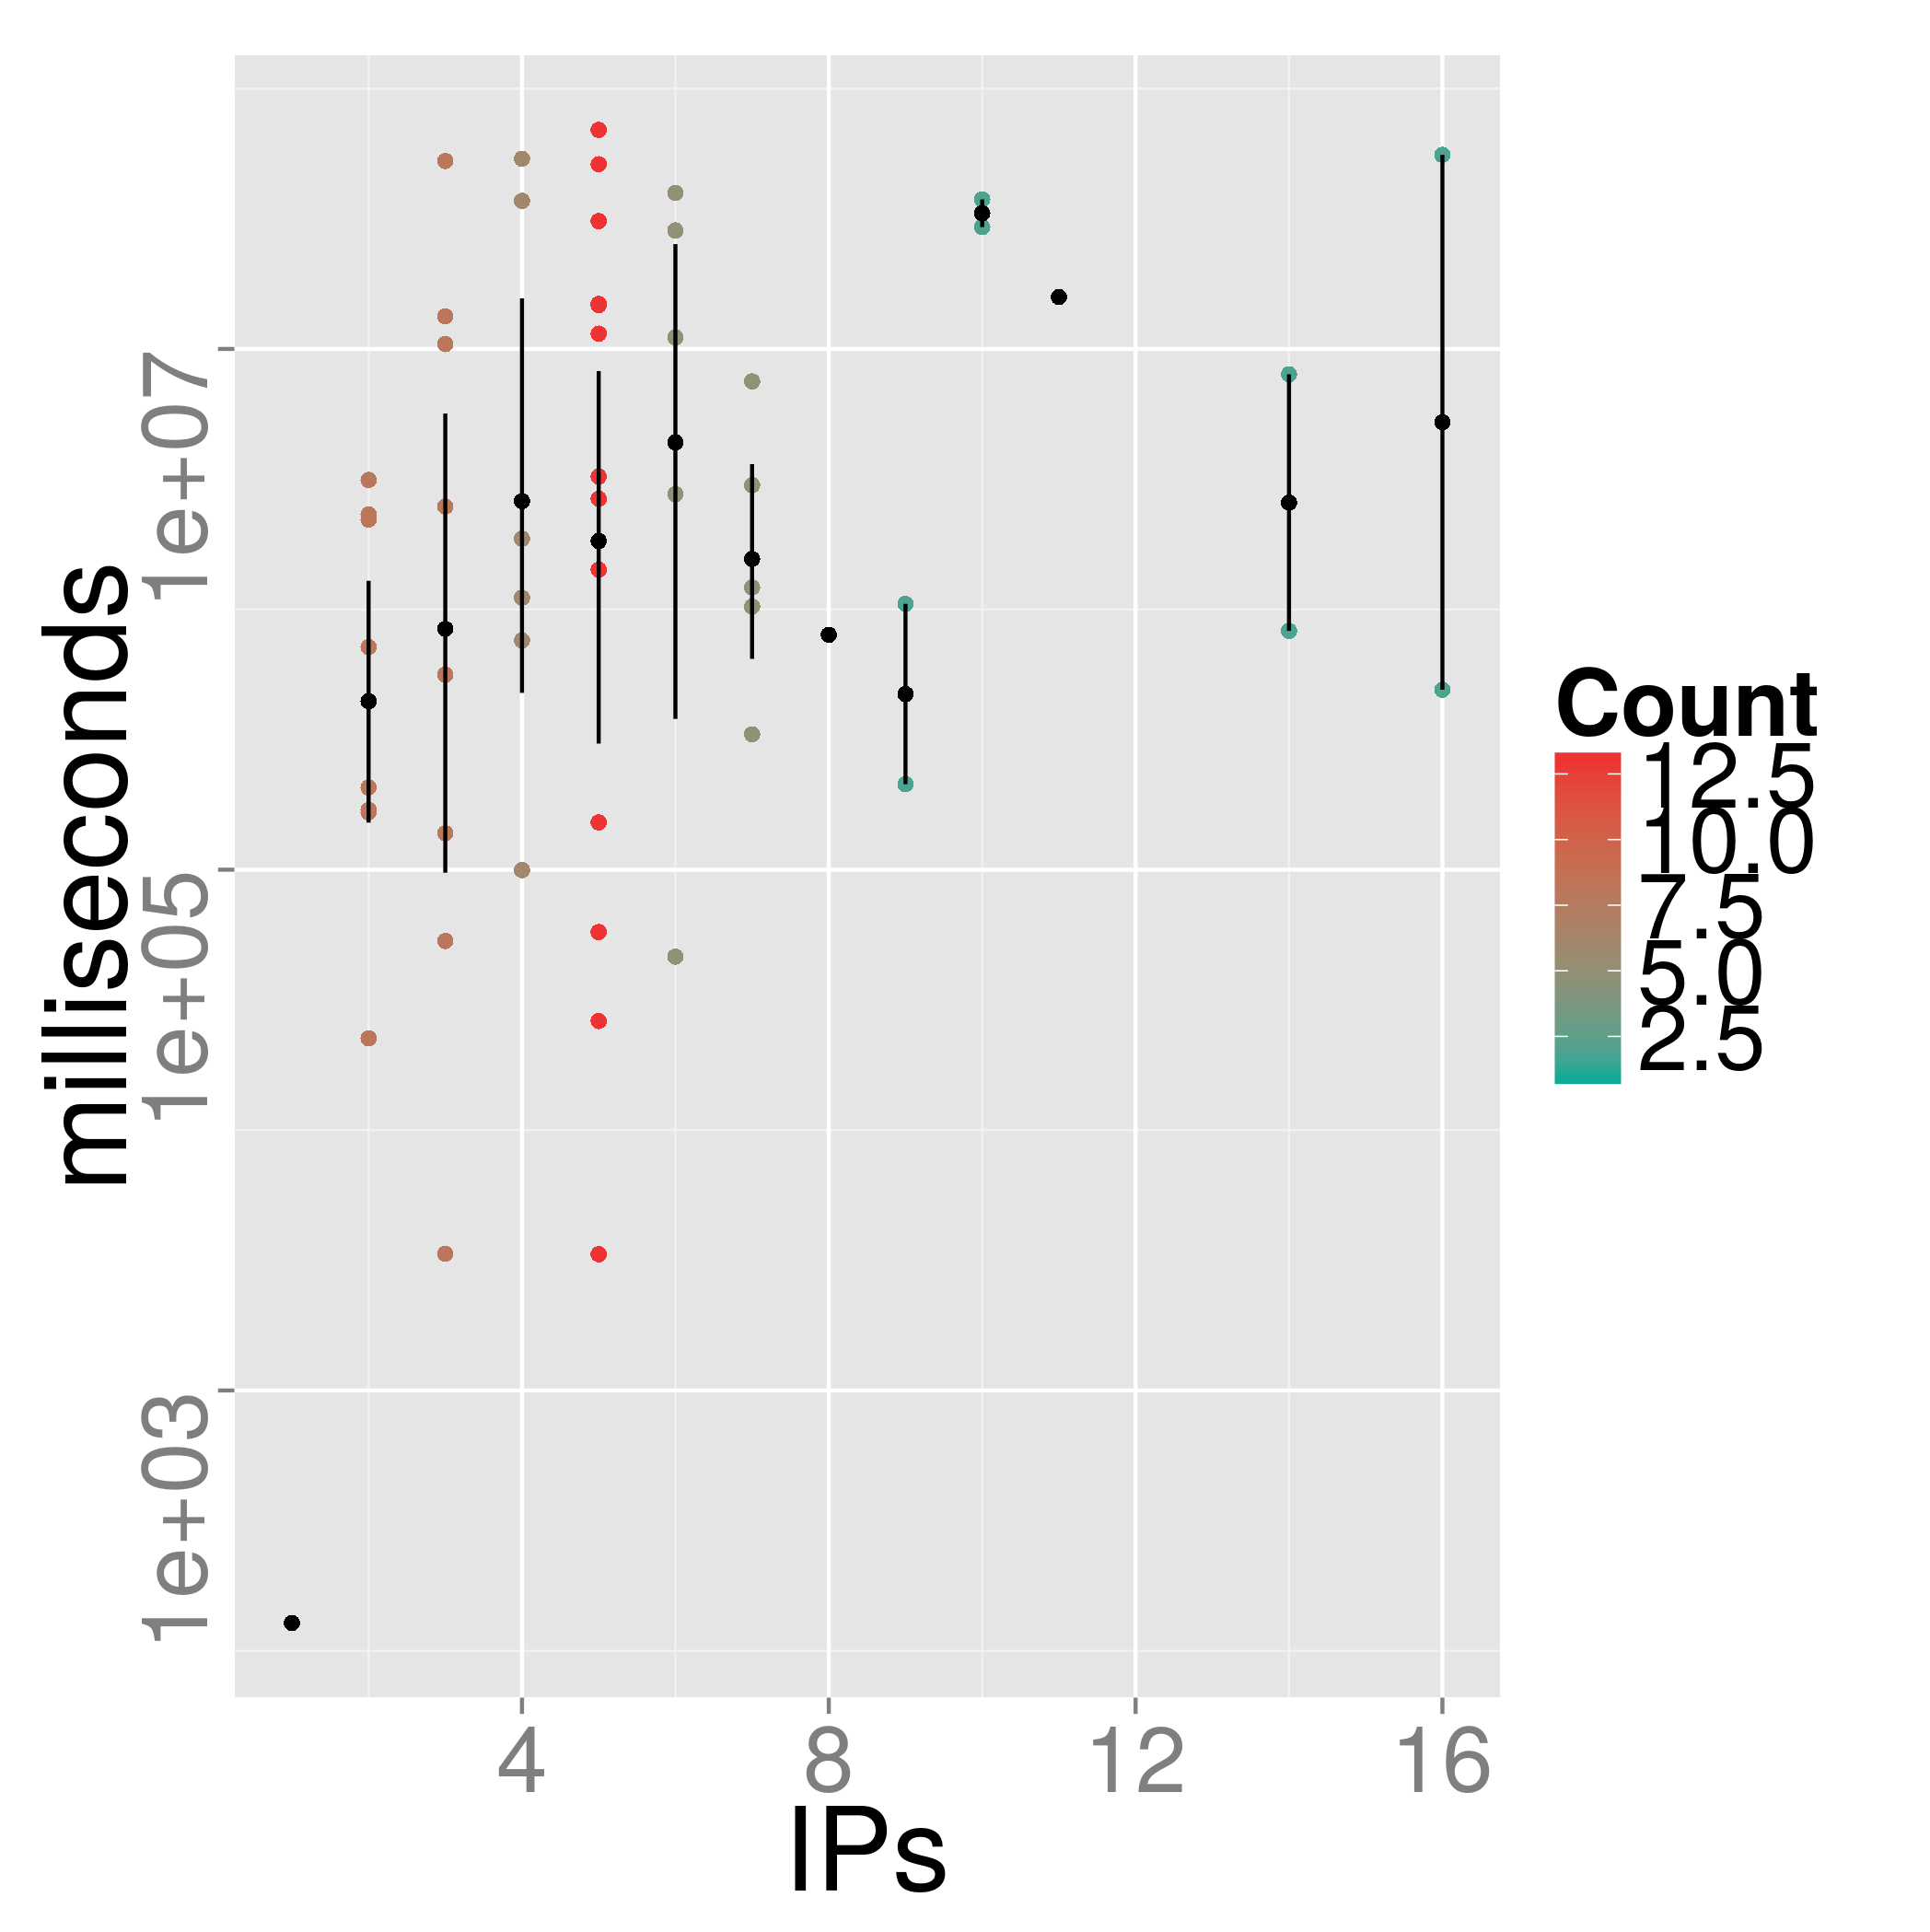
\includegraphics[width=0.32\linewidth]{time-vs-ips-OS-4-4.png}
% 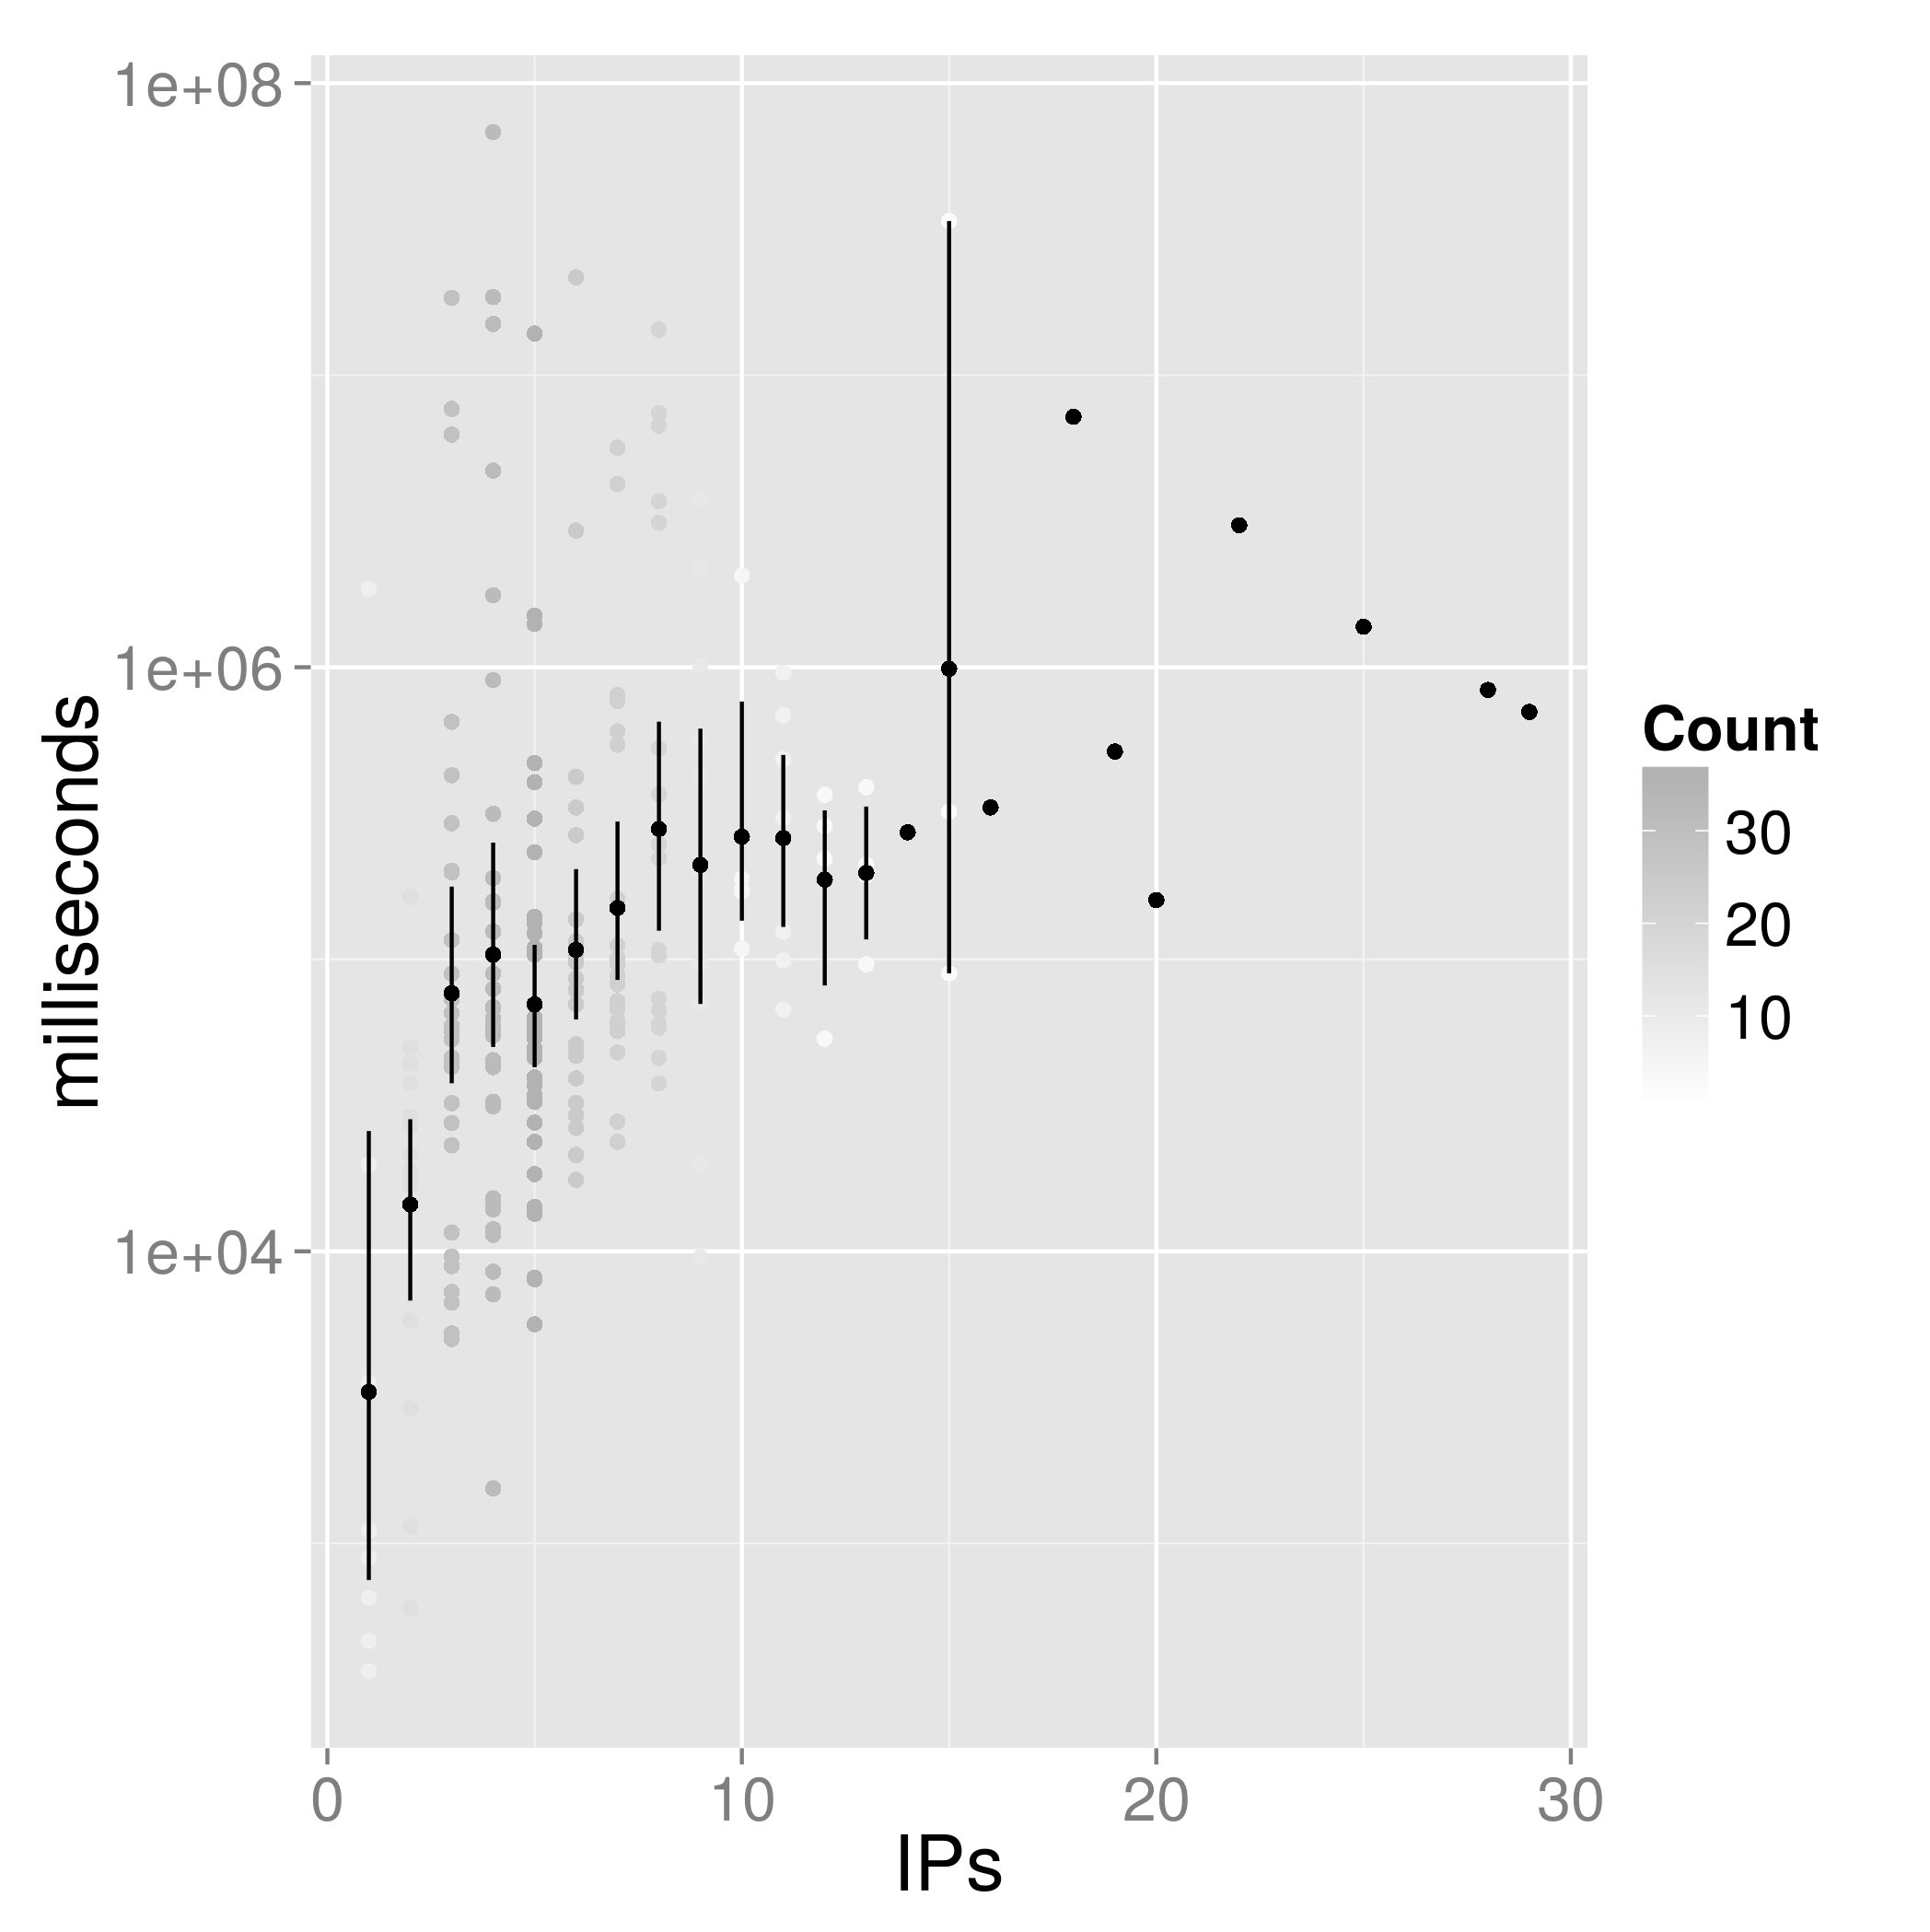
\includegraphics[width=0.32\linewidth]{time-vs-ips-OS-4-24.png}
% 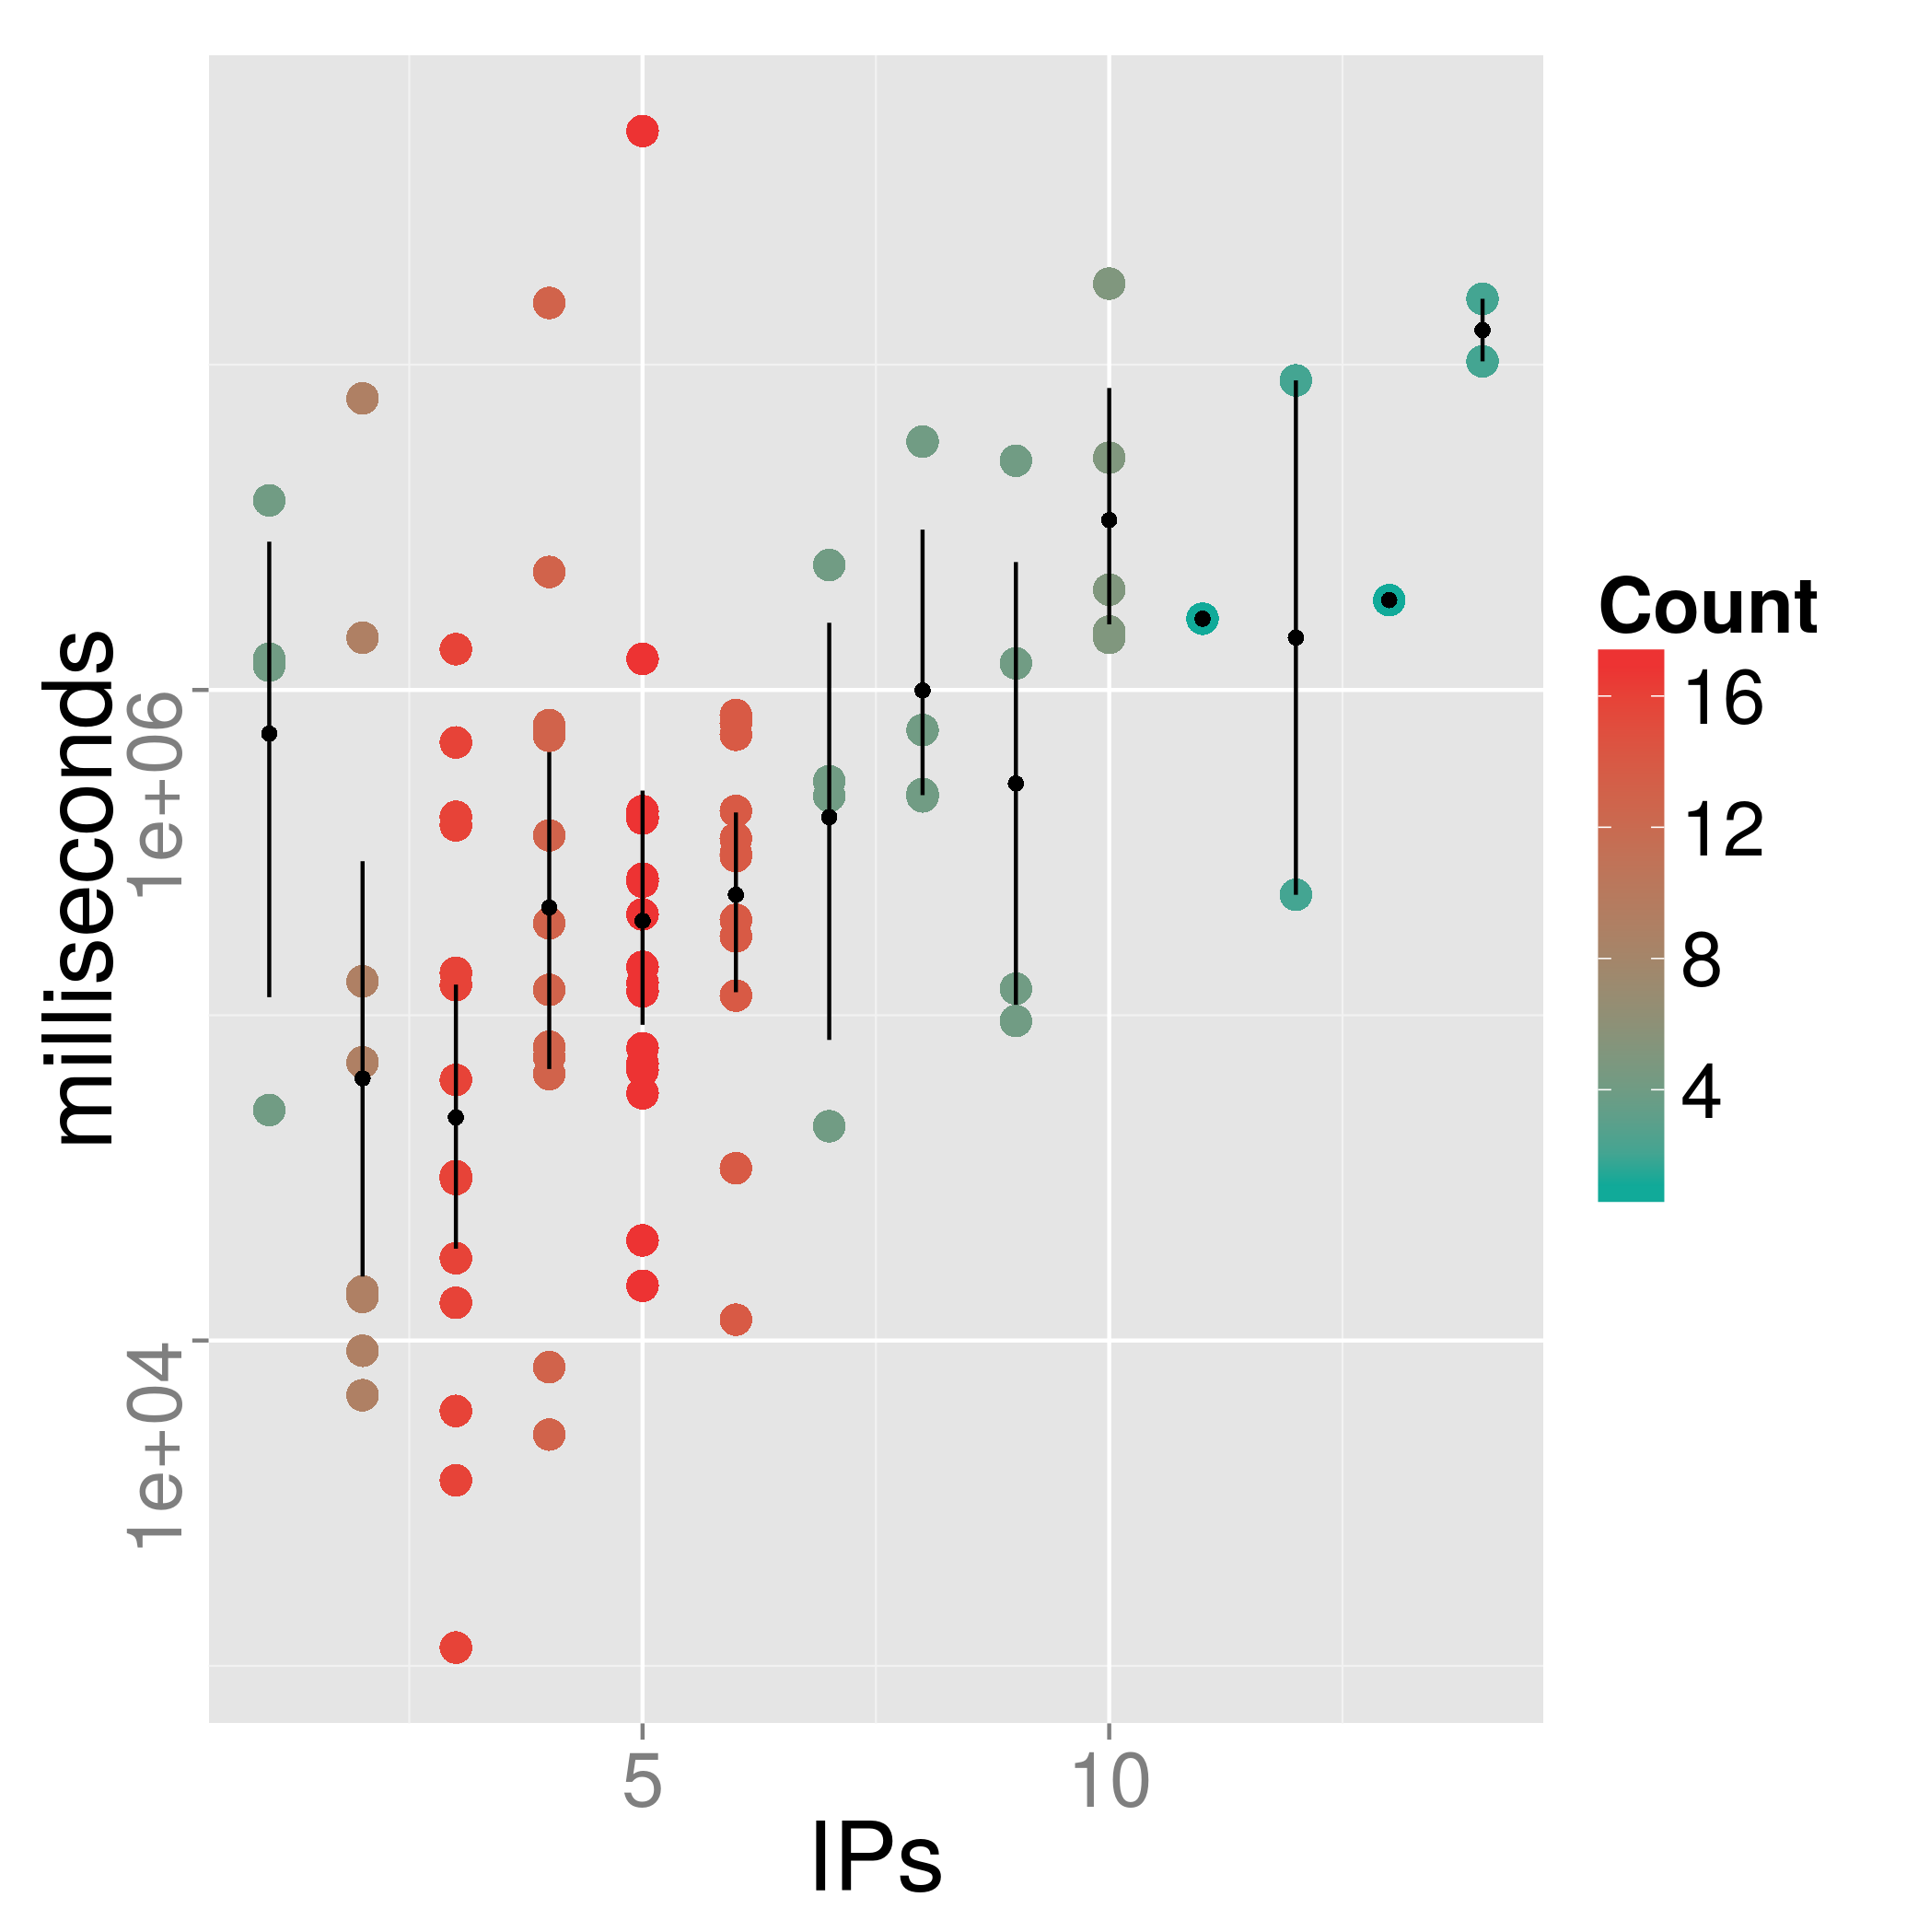
\includegraphics[width=0.32\linewidth]{time-vs-ips-OS-7-31.png}
% \caption{Duration of experiments vs. number of different IPs (nodes)
%   participating in it, with averages and standard deviation shown as
%   black dots and lines, single dot if it was 1). Shade of gray or
%   color indicate how many experiments included that many unique IPs.
% From left to right, experiments 4/4, 4/24 and 7/31.}
% \label{fig:duration}
% \end{figure}
% % ../data/time-vs-IPs-openshift.R
%
\begin{figure}[!htb]
\centering
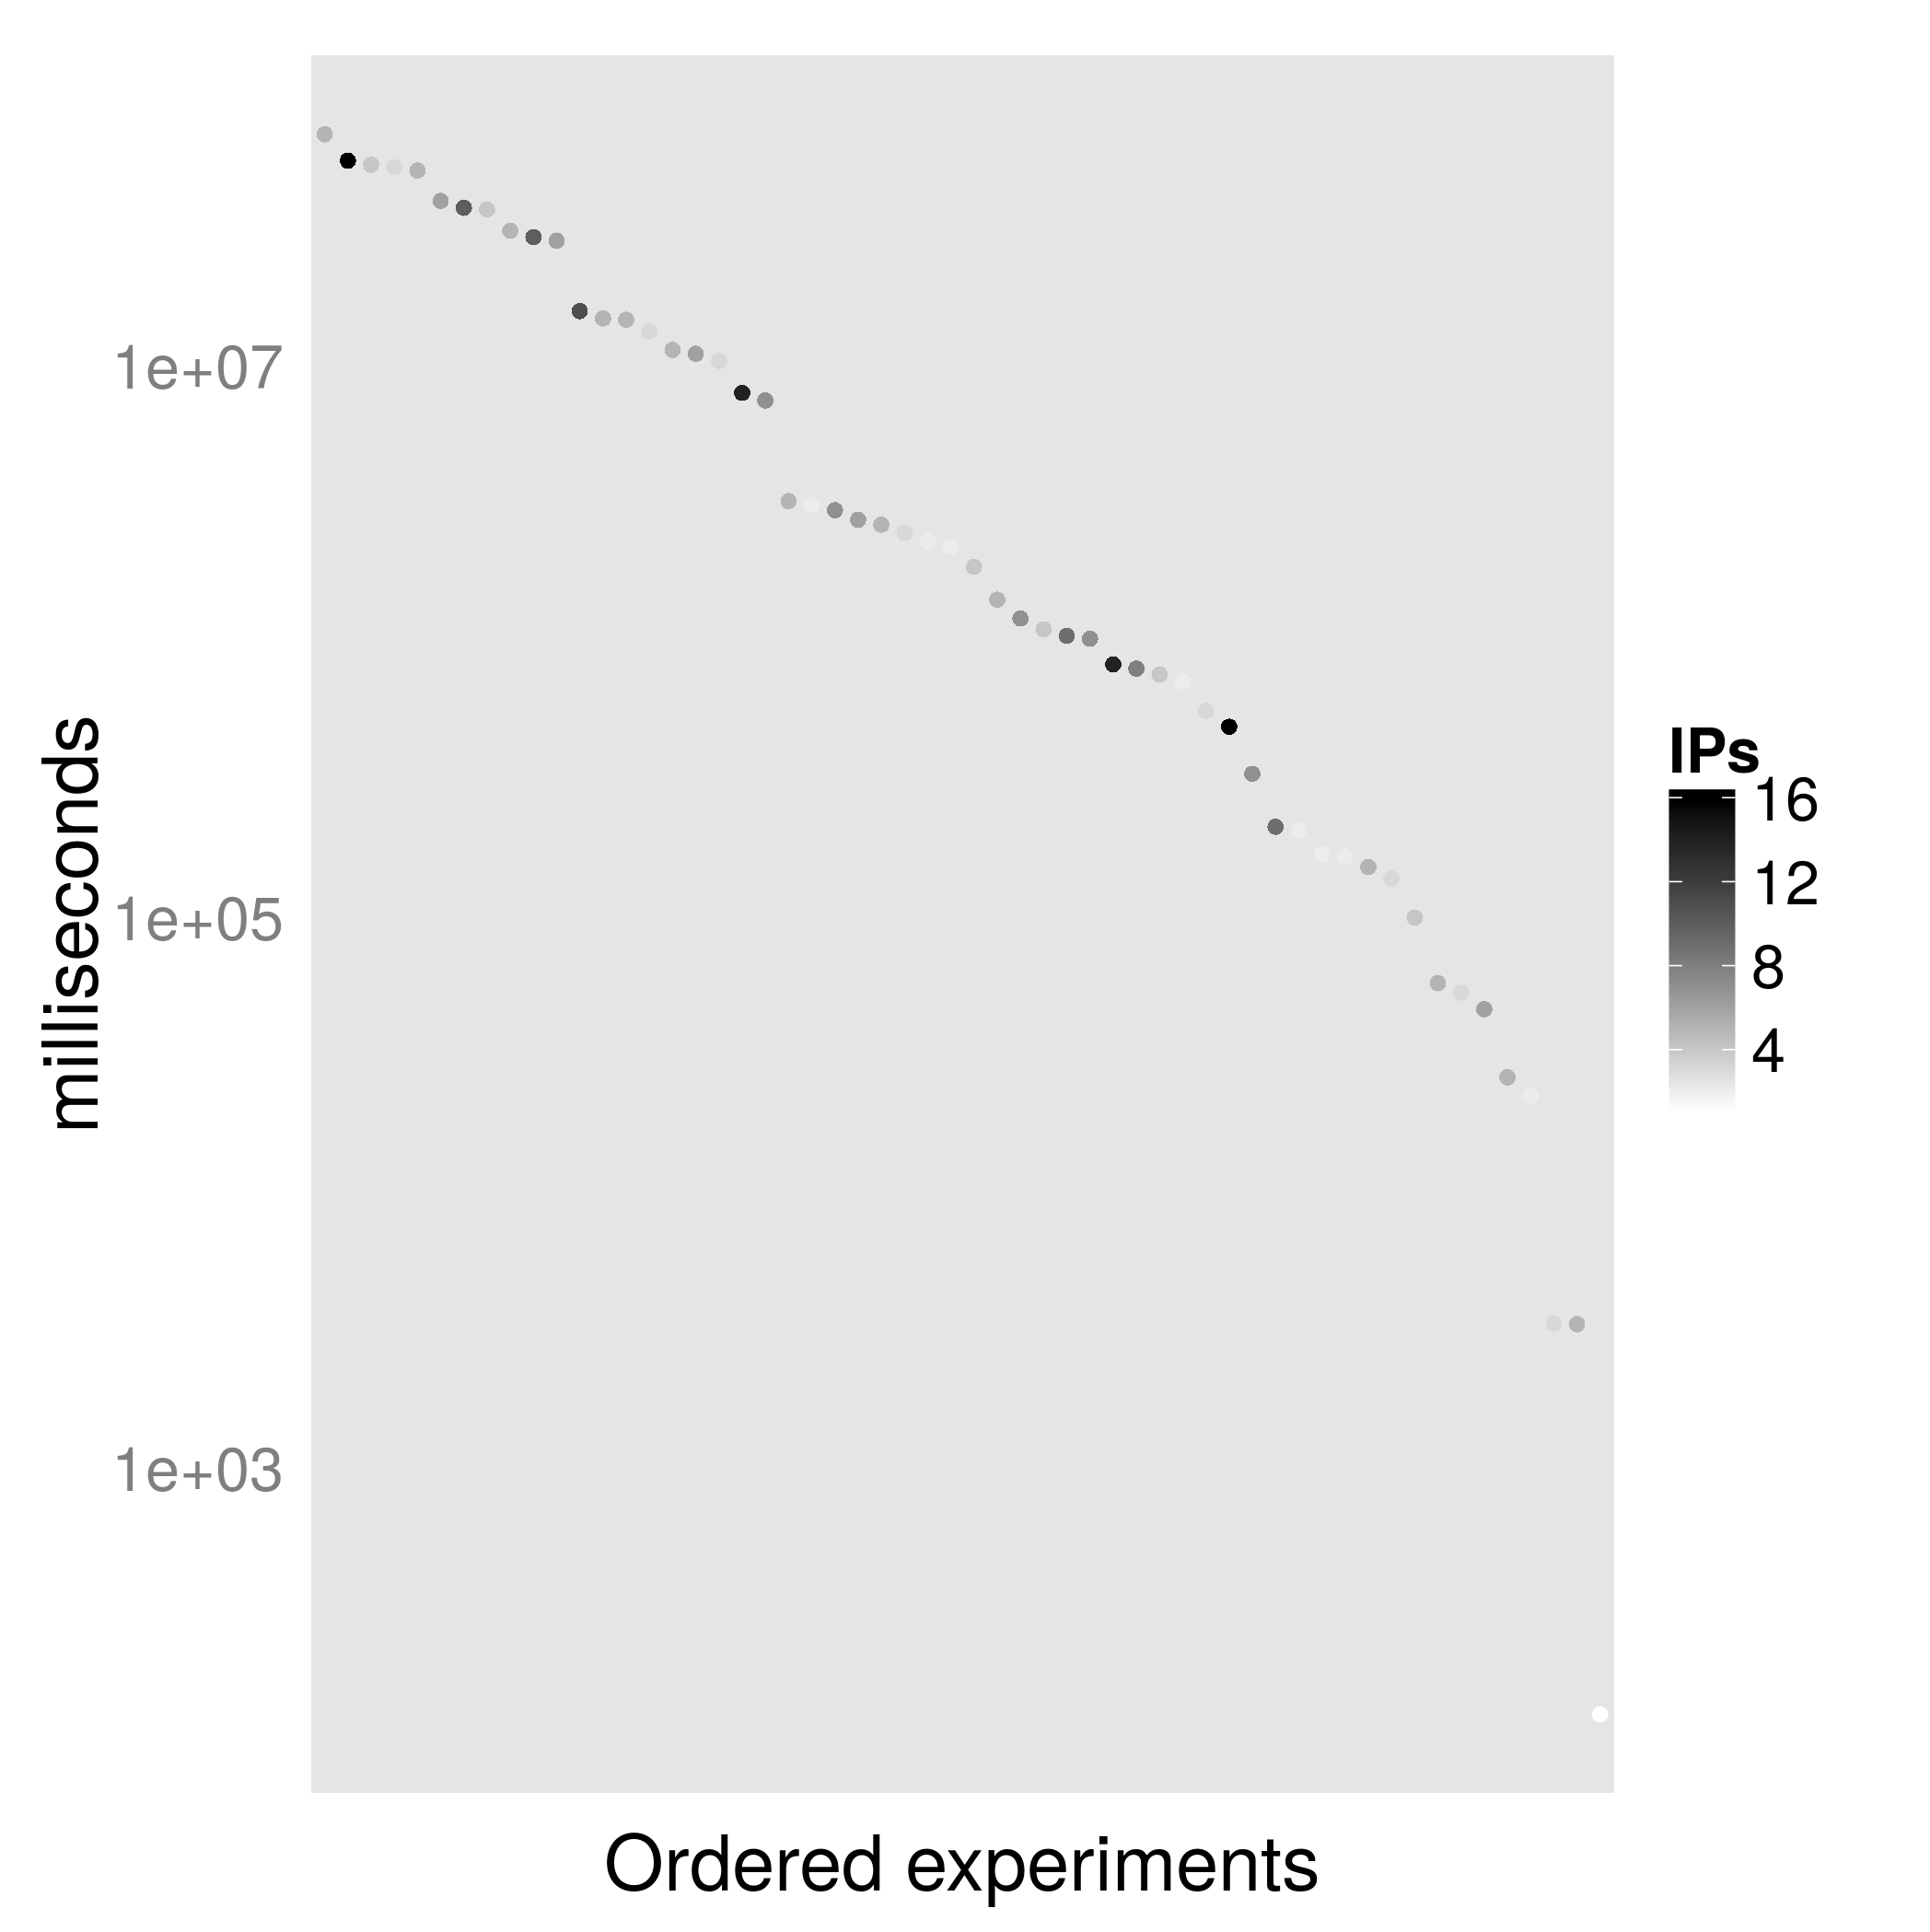
\includegraphics[width=0.32\linewidth]{time-vs-rank-OS-4-4.png}
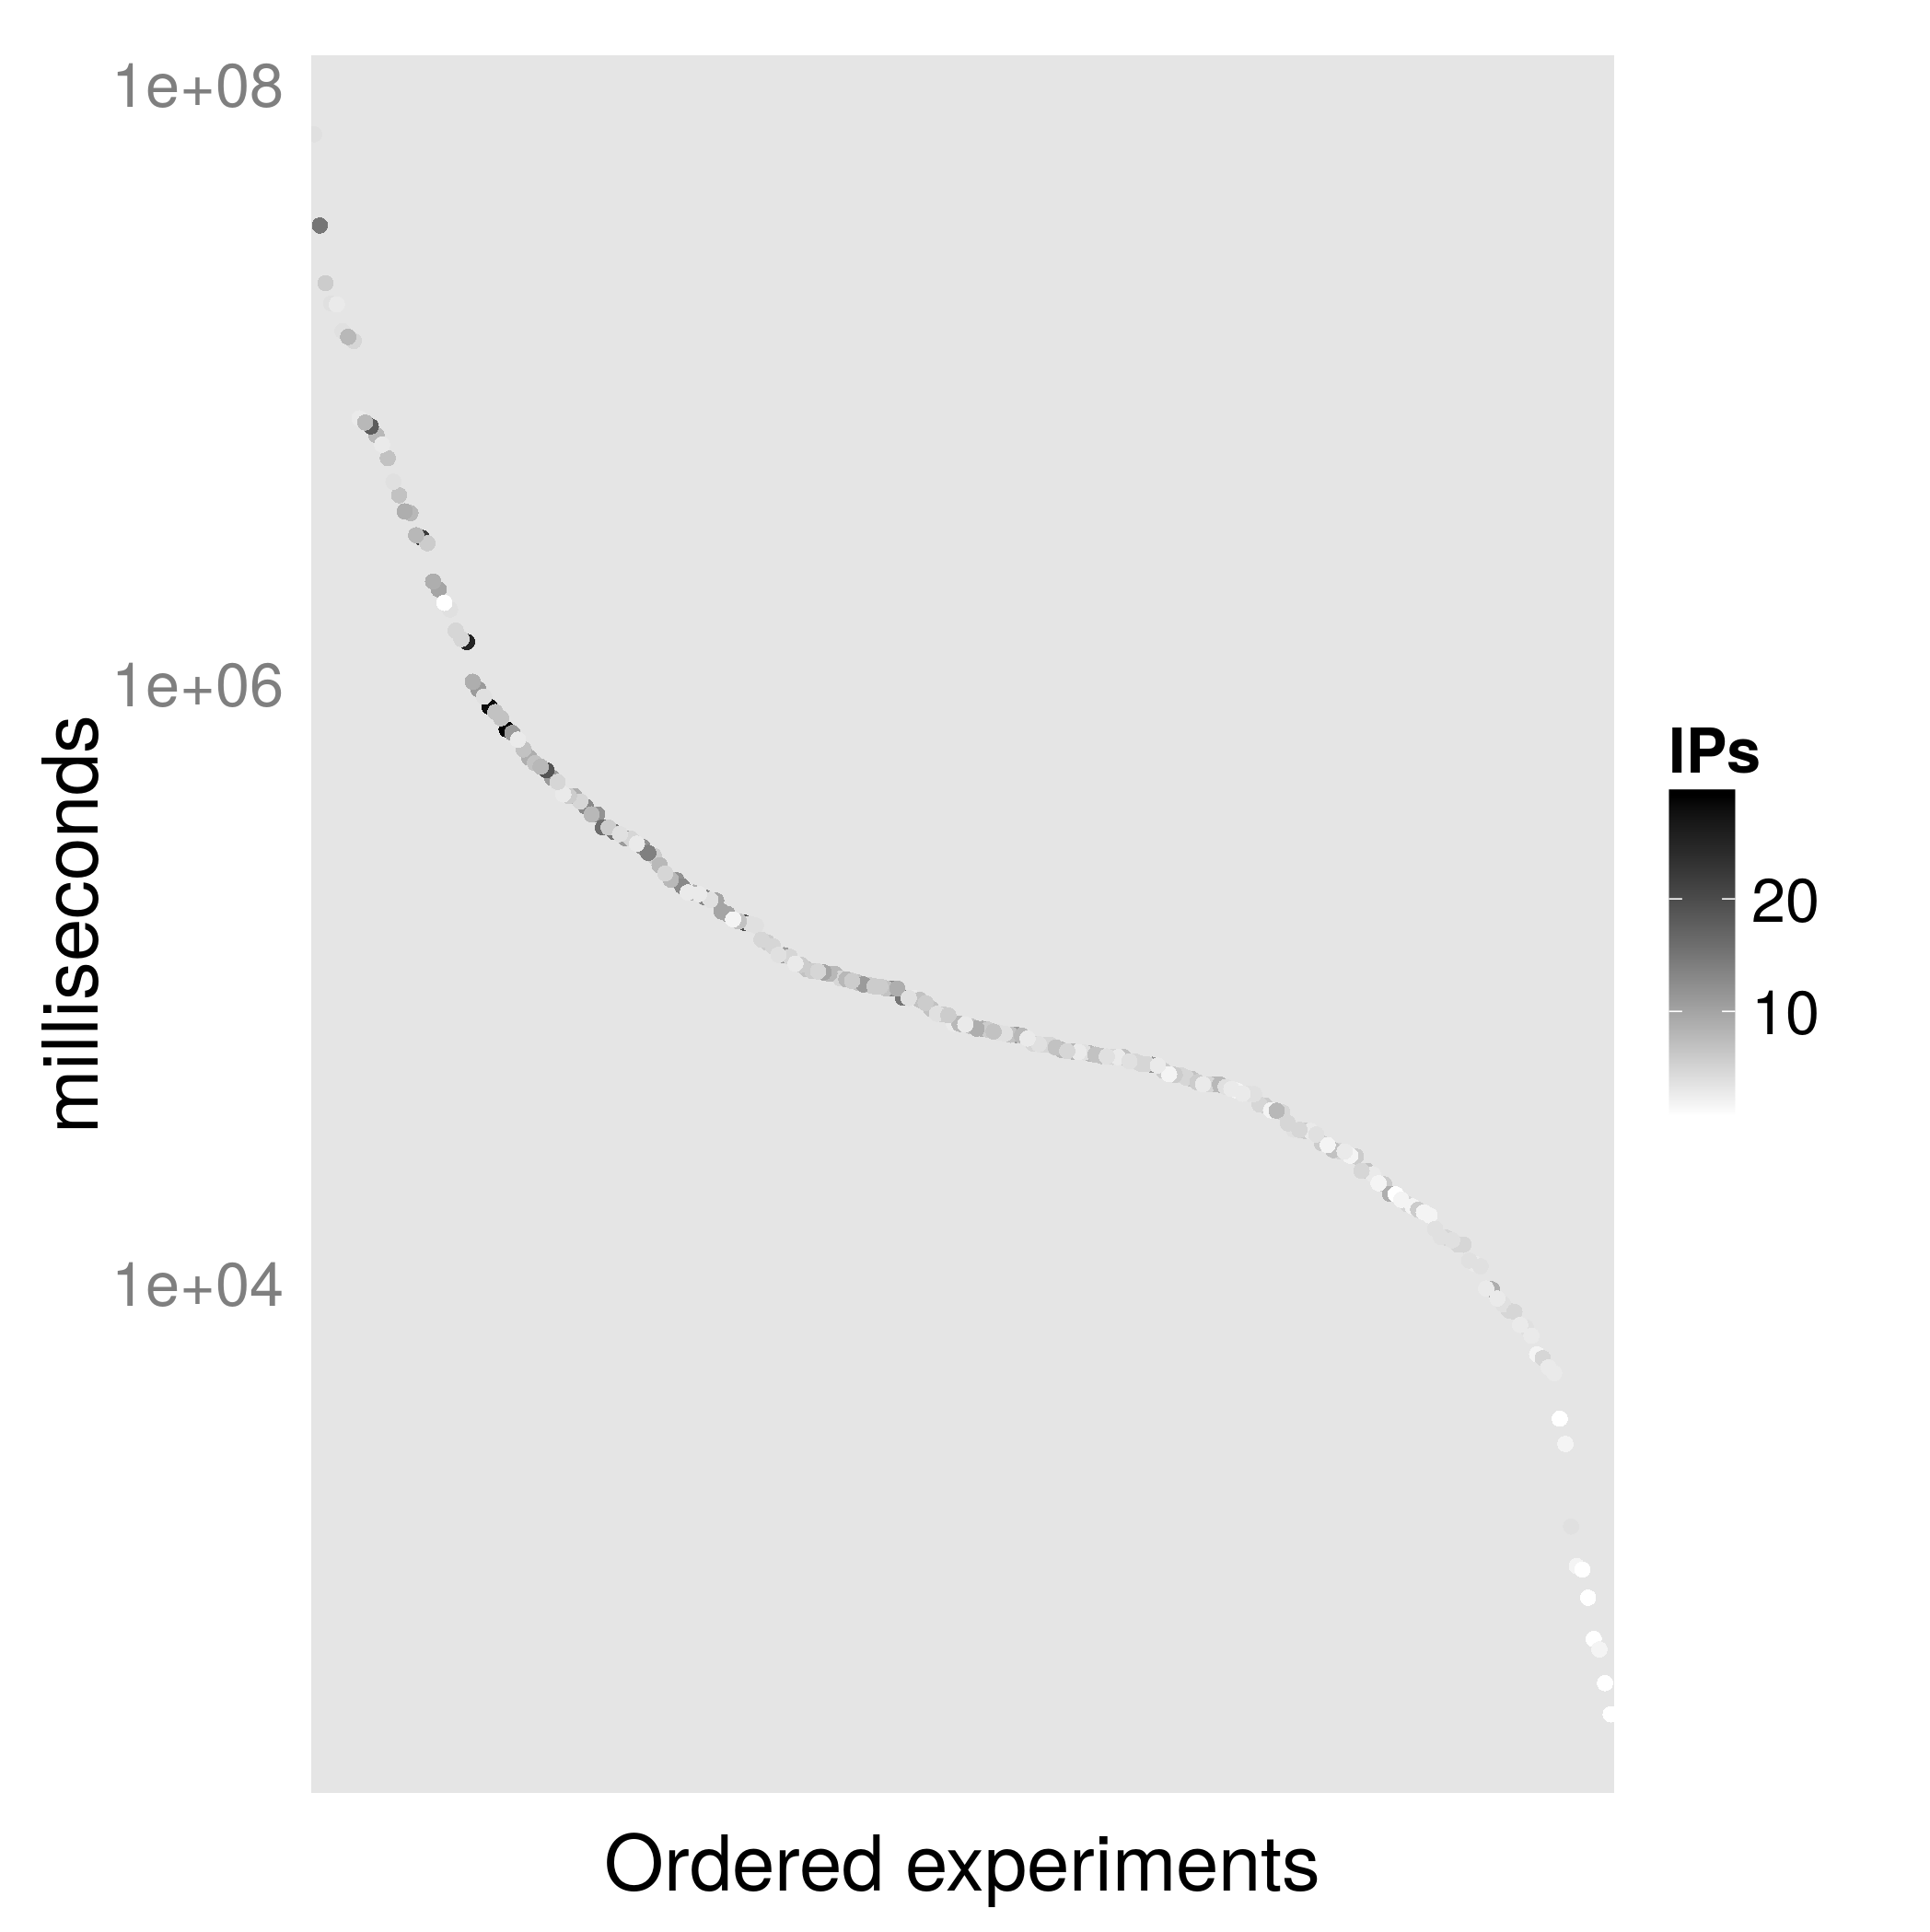
\includegraphics[width=0.32\linewidth]{time-vs-rank-OS-4-24.png}
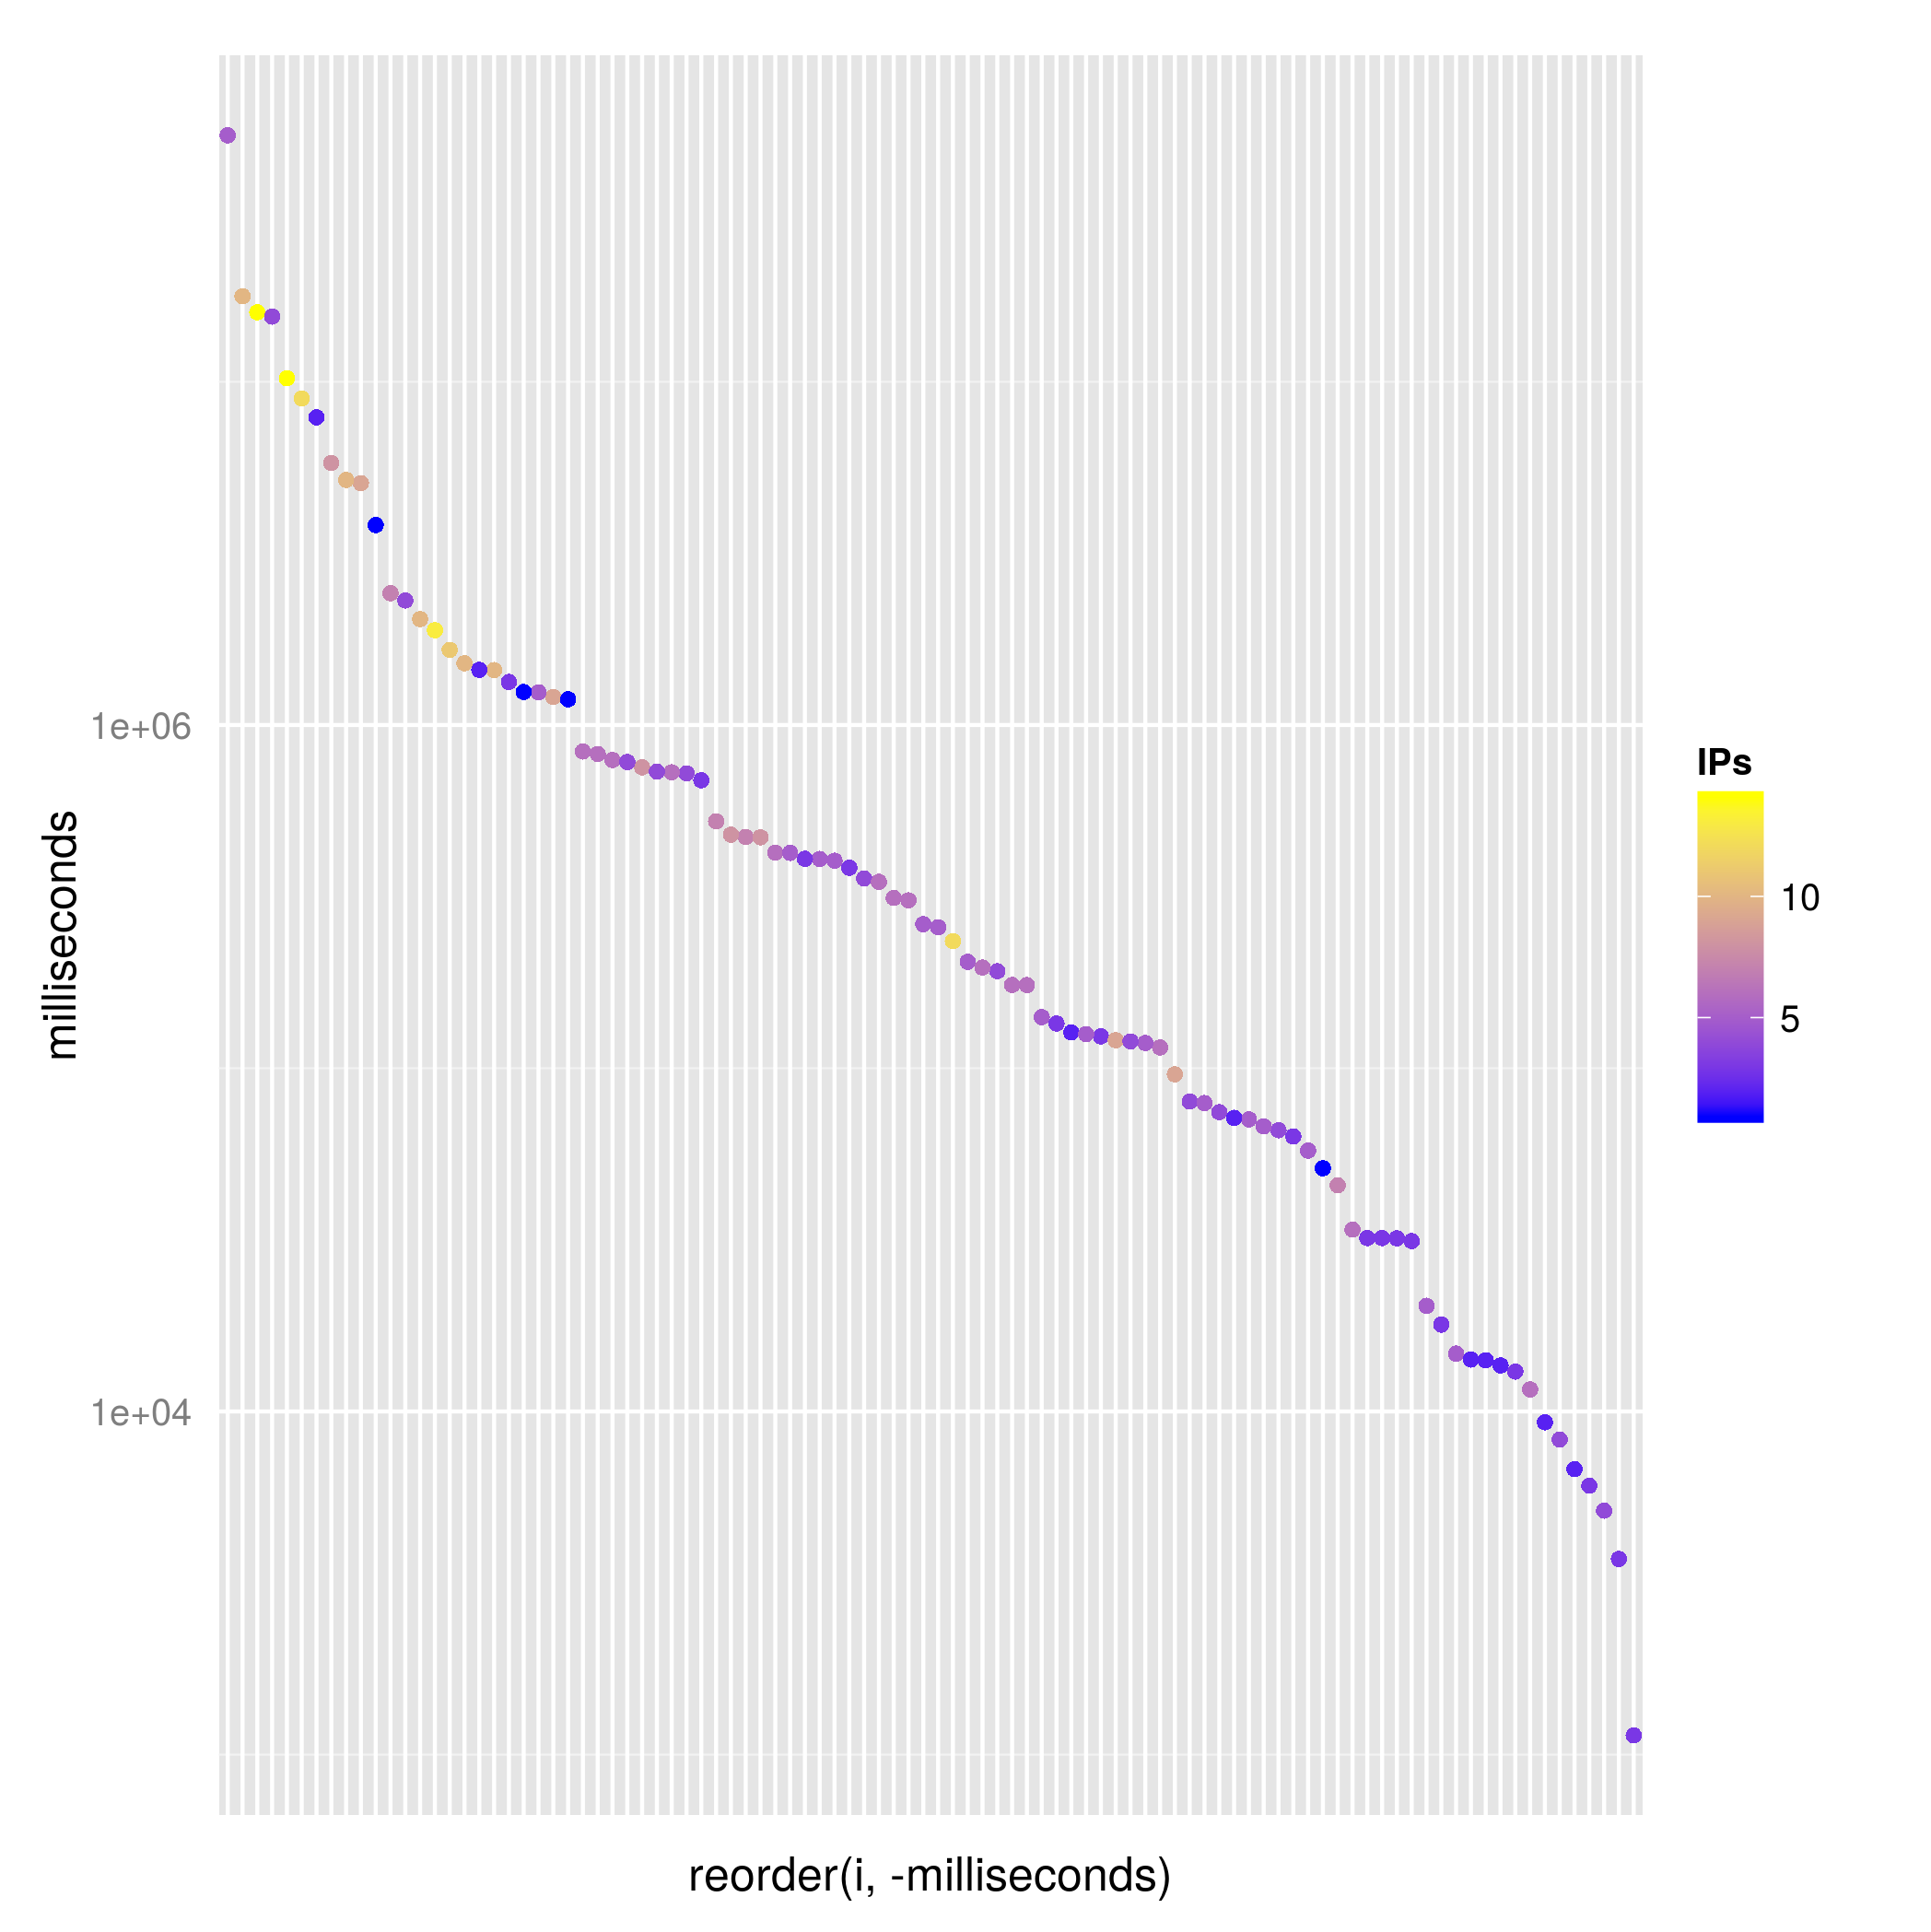
\includegraphics[width=0.32\linewidth]{time-vs-rank-OS-7-31.png}
\caption{Duration of experiments vs. rank, with $y$ axis in a
  logarithmic scale. Dot color (or gray value) is related to the number of IPs
  participating in the experiment. From left to right, experiments
  4/4, 4/24 and 7/31.} 
\label{fig:zipf:os}
% computed via ../data/time-vs-IPs-openshift.R
\end{figure}
%
% We will have to analyze experimental data a bit further to find out why
% this happens and also if there are some patterns in the three sets of
% experiments. An interesting question to ask, for instance, is if
% by adding more computers makes the experiment take less. In fact, as
% shown in Figure \ref{fig:duration}, the {\em addition} of more computers does
% not seem to contribute to decreasing the time needed to finish the
% experiment. However, the cause-effect relationship is not clear at
% all. It might be the opposite: since experiments take longer to finish
% and might in fact be abandoned with no one contributing for some time,
% that increases the probability of someone new joining them. In fact,
% with experiments taking a few seconds and due to the way the
% experiments are announced, it is quite difficult that several
% volunteers join in in such a short period of time, even more if we take
% into account that volunteers are not {\em carried over} from previous
% experiments. This implies that it would be convenient to use a problem
% of a bigger size to check this hypothesis as we have done in the next
% experiment. 
%  However, at this point we
% have not found this convenient since there are several other issues
% that have to be solved, as it will be shown next. %Creo que este párrafo
%saldría sobrando ahora que hicmios un experimento más grande

\begin{figure}[!htb]
\centering
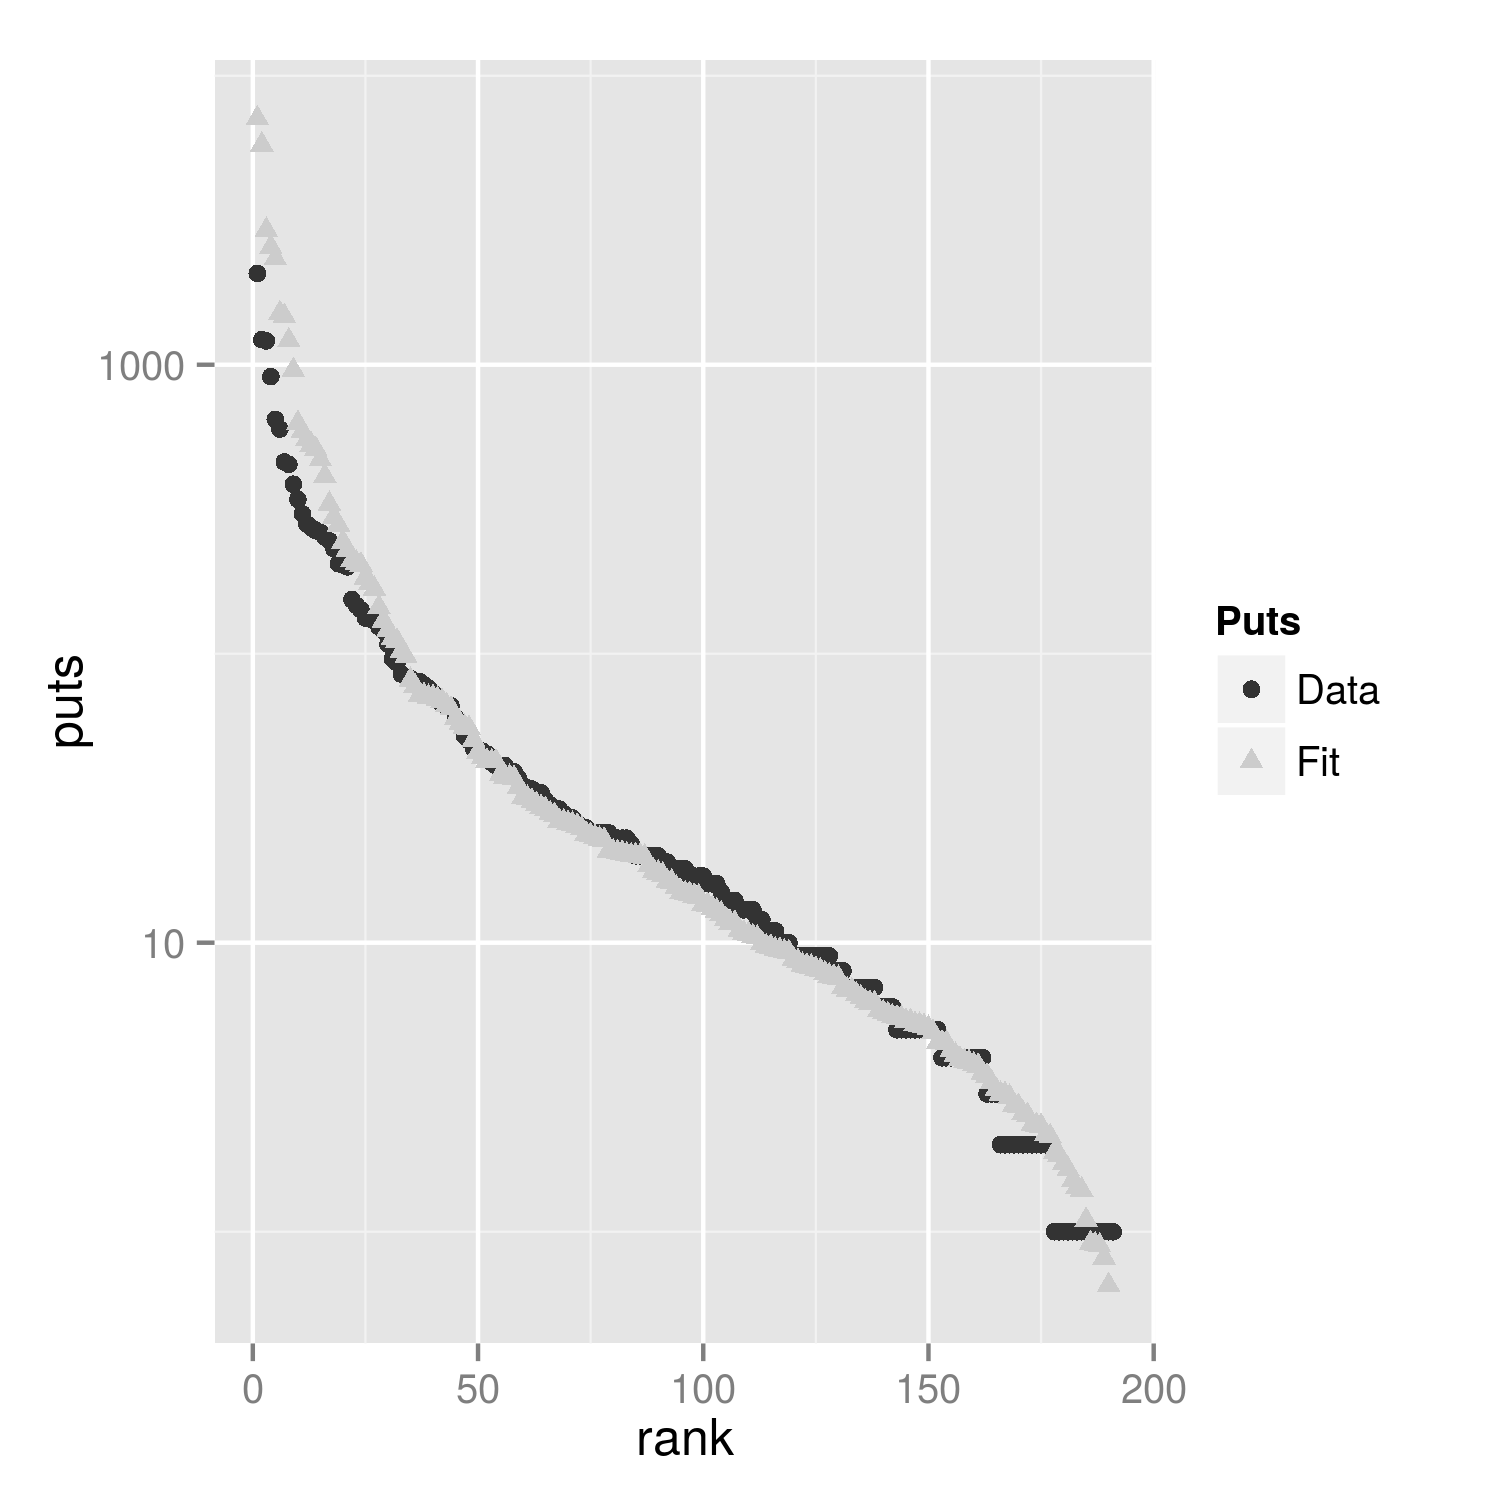
\includegraphics[width=0.32\linewidth]{puts-openshift-4-4.png}
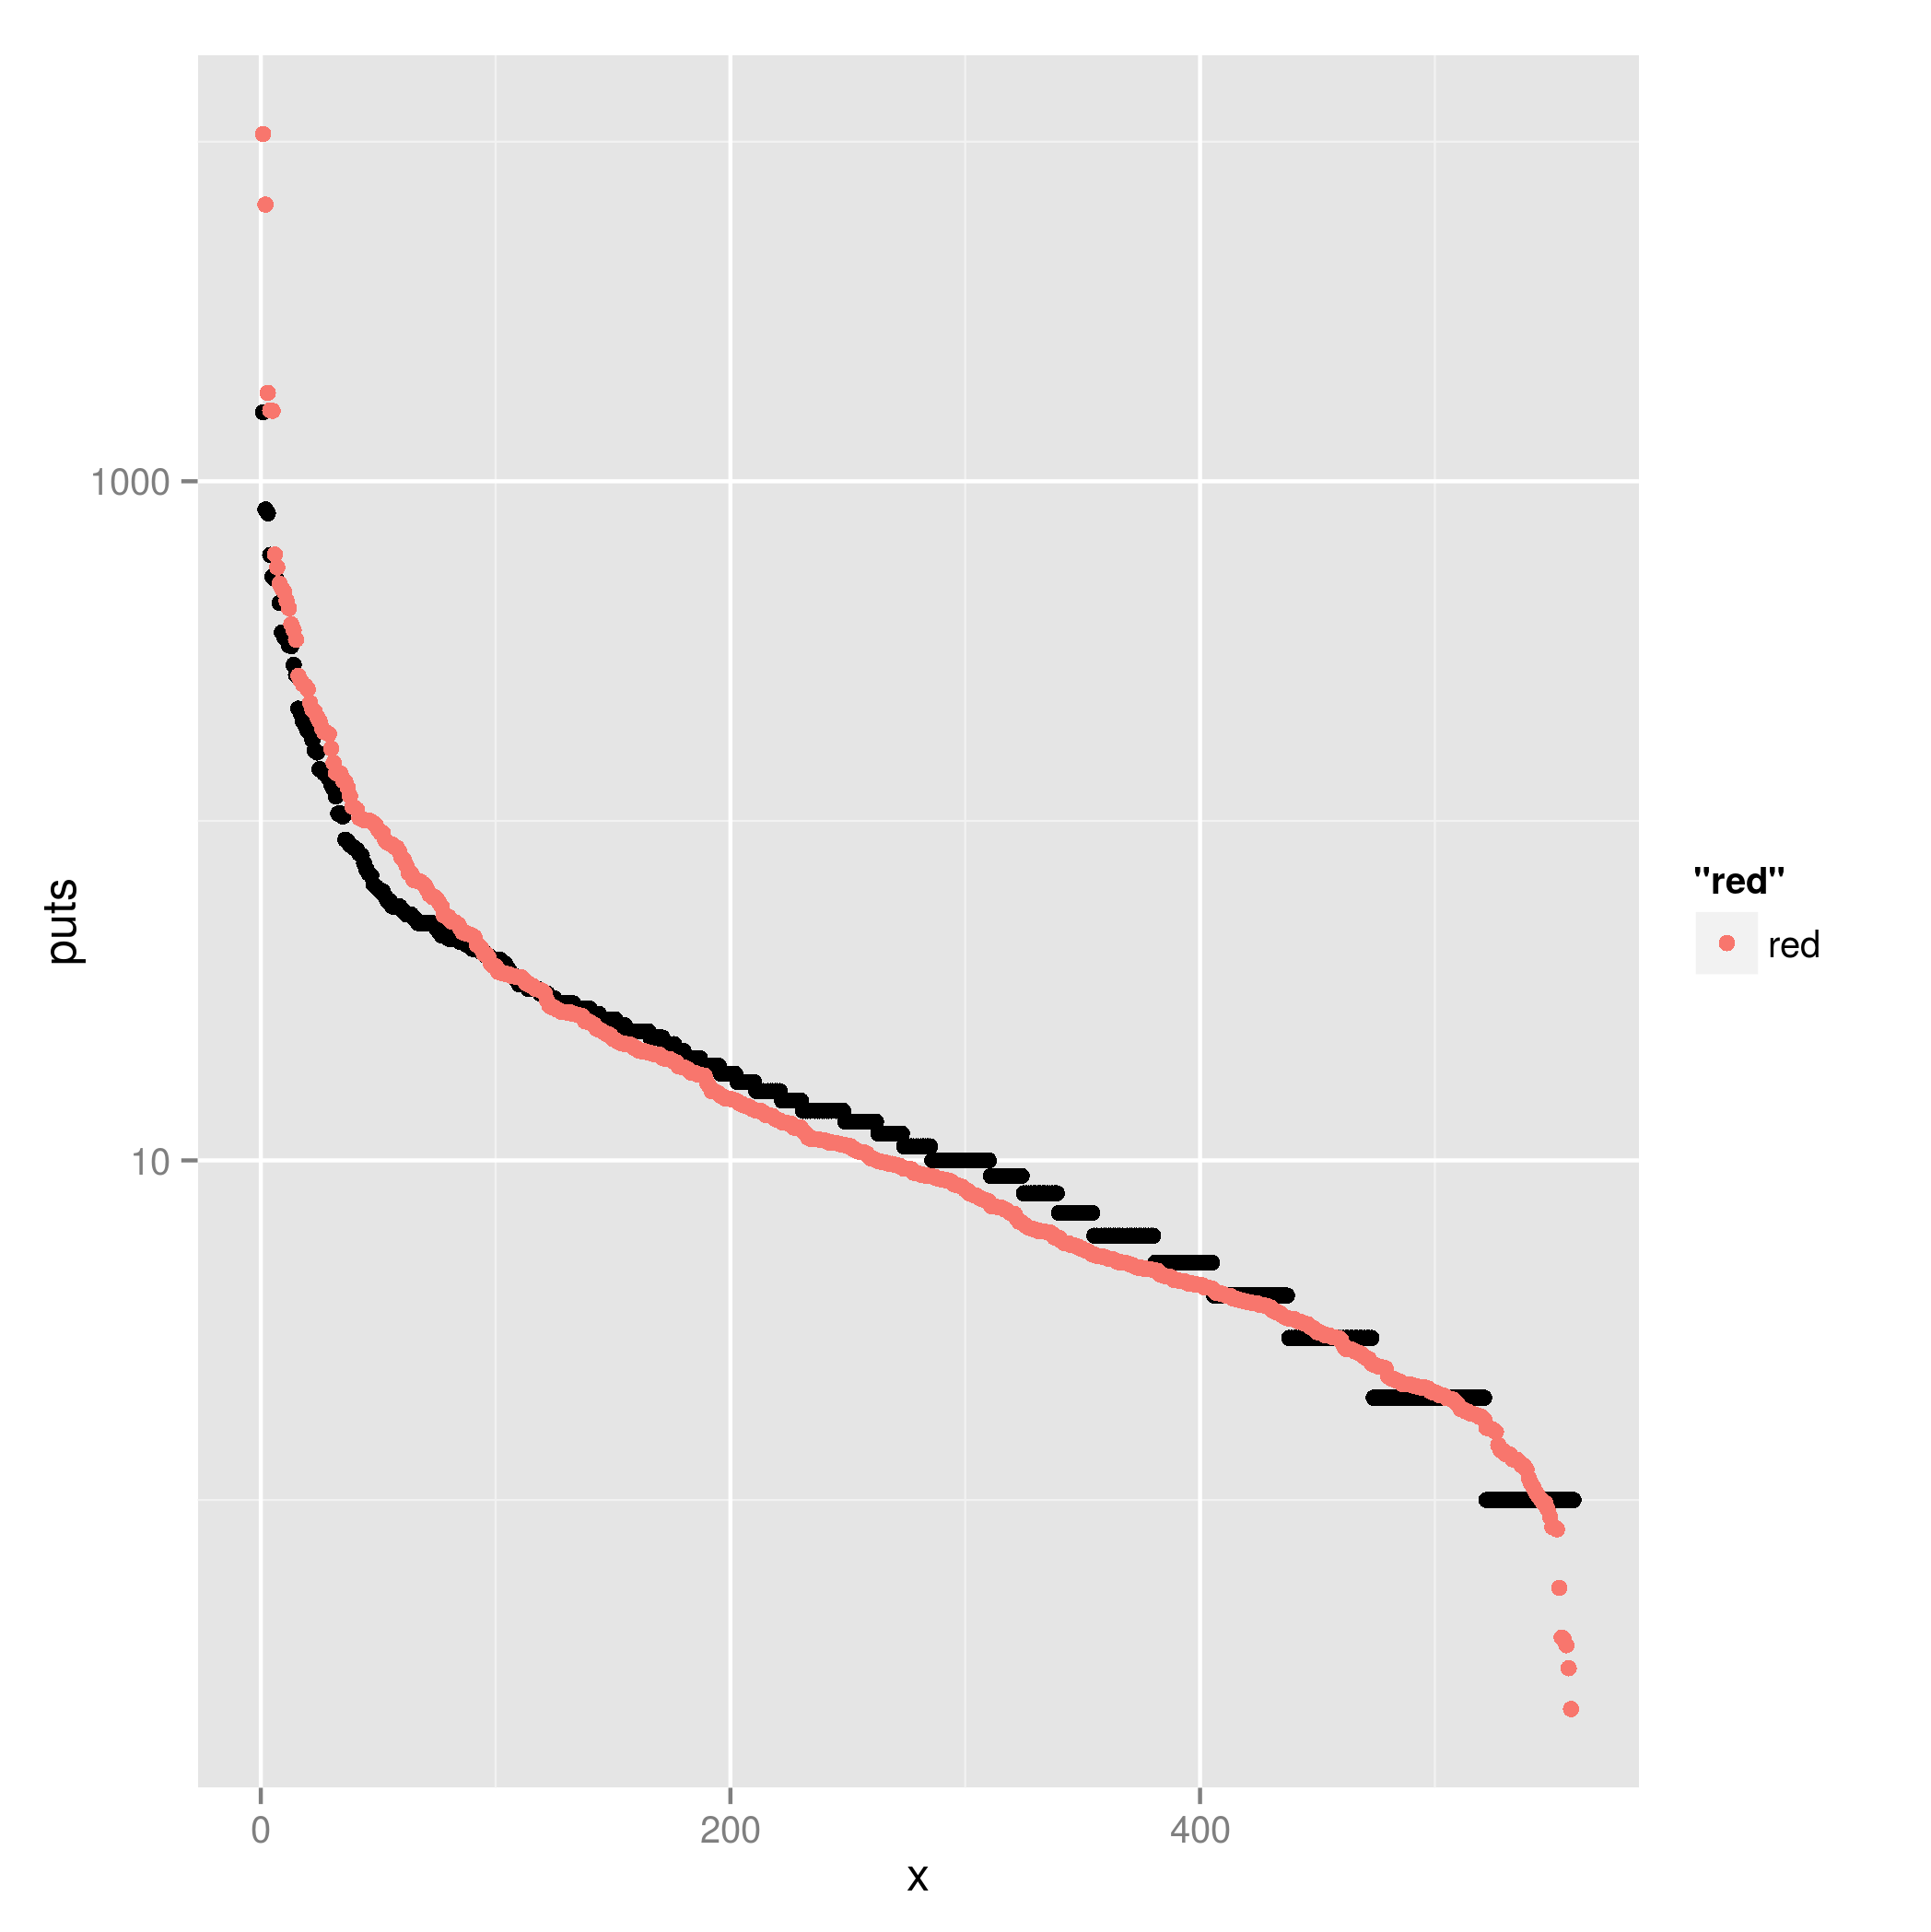
\includegraphics[width=0.32\linewidth]{puts-openshift-4-24.png}
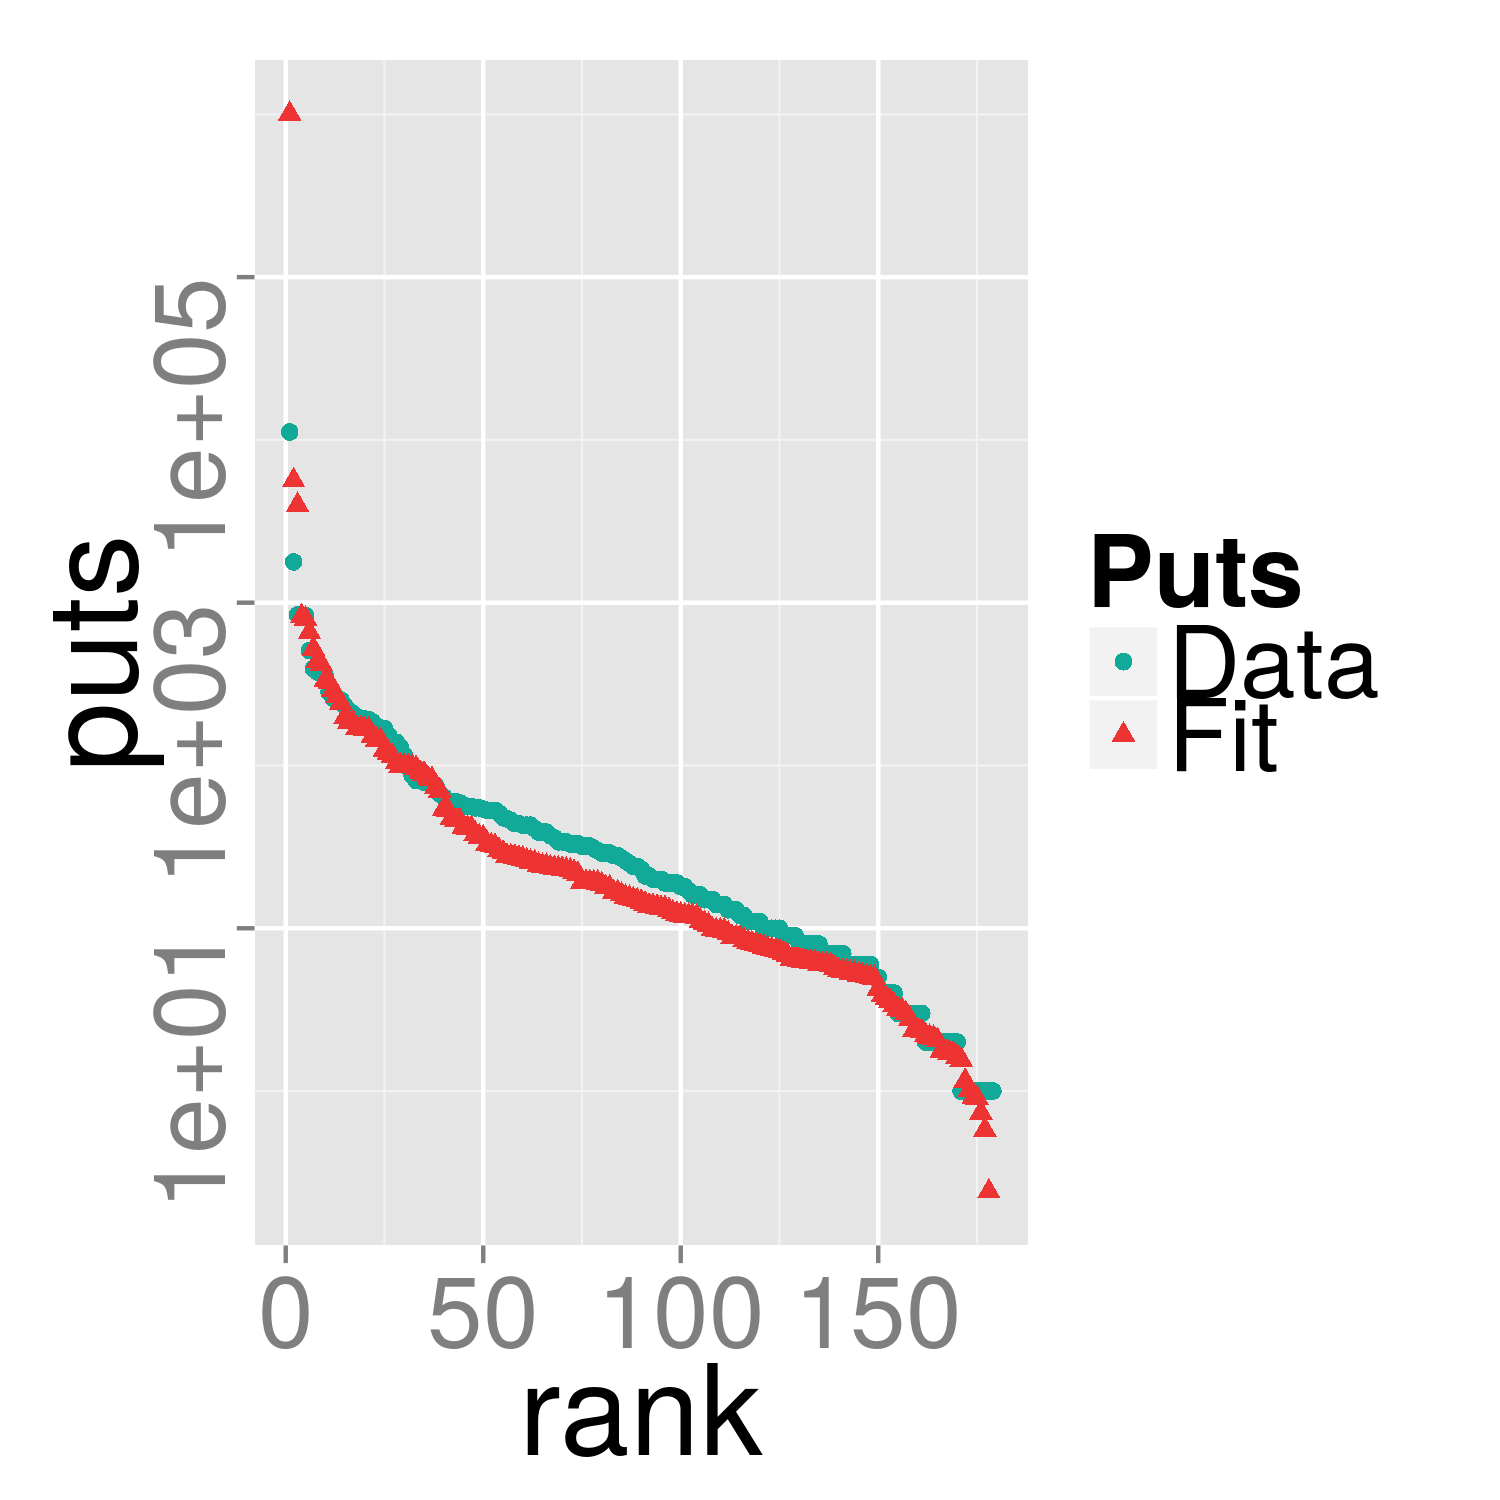
\includegraphics[width=0.32\linewidth]{puts-openshift-7-31.png}
\caption{Number of PUTs per unique IP and fit to a Generalized
  Extreme Value distribution (in a lighter shade or blue). From left to right, experiments
  4/4, 4/24 and 7/31.} 
% Plotted with ../data/plot-zipf-openshift.R
\label{fig:puts:os}
\end{figure}
%
It is also interesting to check the distribution of the experiment
duration, shown in Figure \ref{fig:zipf:os} and which roughly follows
a Zipf's law, with similar distribution along all three runs. The 4/24
run is the most complete and shows an S-shape, which implies an
accumulation of experiments taking similar time and around 100
seconds. The most interesting part is the {\em tail}, which shows how
many experiments took a desirable amount of time, on the order of
10 seconds, and which appears in all three graphs. As it can be seen,
it sharply drops implying there are 
just a few of them, and with diminishing probability as time
decreases. This exponential distribution also appears in Figure \ref{fig:puts:os}, which shows the
distribution of HTTP PUTs, equivalent to the number of
generations divided by 100, contributed by every user. These results show a Zipf-like behavior,
so we have fitted it to the Generalized Extreme Value distribution,
with the resulting parameters shown in Table \ref{tab:puts:os}.
%
\begin{table}
\caption{Summary of fit to Generalized Extreme Value distribution of
  the number of PUTs per unique IP. \label{tab:puts:os}}
\begin{center}
\begin{tabular}{l|ccc}
\hline
Date  & Location $\mu$ & Scale $\sigma$ & Shape $\xi$ \\
\hline
4/4 &  8.541 $\pm$ 1.0926  &    12.442 $\pm$ 1.7302 &  1.388 $\pm$
0.1377 \\
4/24 & 6.148 $\pm$ 0.3782 & 7.354 $\pm$ 0.5105 & 1.090 $\pm$  0.0697  \\
7/31 & 11.645 $\pm$ 1.475 & 16.365 $\pm$ 2.201 &  1.265 $\pm$ 0.132   \\
\hline
\end{tabular}
\end{center}
\end{table}

This distribution was originally proposed to fit extreme values
\cite{resnick2013extreme} and contains, as a special case, the inverse
Weibull distribution which was fitted to volunteer computing
frameworks such as SETI@home \cite{javadi2009mining}. We obviously do
not pretend to compare our framework in scale or complexity with it, but
to point out that the behavior of volunteer computing nodes follows a
certain pattern, found in SETI@home, and which also appears in our
framework. 

This
distribution is governed by three parameters, the usual location $\mu$
which is related to where it has its {\em center} and a scale $\sigma$,
related to the size, but also a third shape $\xi$ parameter that is
related to its skewness, that is, how skewed it is around the central
location. Positive parameters indicate that the distribution {\em
  leans} towards the origin, and negative ones towards the other extreme
value. In this case, Table \ref{tab:puts:os} shows $\xi$ values
greater than one and between one and 1.4, which indicates that the
three experiments share this origin-leaning pattern, with many users
donating a few cycles and just a few donating extreme values. Random
distributions with these parameters have been plotted in red in
Figure \ref{fig:puts:os}, indicating that the fit is good enough. The
predictive value of these fits, however, is limited, over all taking
into account the low correlation between successive events which is
shown in the figures afigure bove. 

At any rate, this also shows that a convenient way of increasing the
computing power would be to try and improve this minimum amount of experiments
per user. This is checked next. 

\begin{table*}[!htb]
\caption{Summary of {\sf NodIO-W$^2$} (an acronym for the version that
  uses web workers) and comparison with the previous
  experiments, which have been aggregated to compute central measures. \label{tab:summary:ww}}
\begin{center}
\begin{tabular}{l|ccccccc}
\hline
Date & Median \#IPs & Max \#IPs & Median time (s) & Median \# PUTs & $<$ 69s & $<$ 3.46s & Inter-experiment correlation\\
\hline
{\sf NodIO} & 5 & 29 & 123 & 14 & 37.43\% & 3.40\% & 0.10 \\
{\sf NodIO-W$^2$} & 4  & 16 & 7.36 & 40 & 89\% & 36.90\% & 0.4336061 \\
\hline
\end{tabular}
\end{center}
\end{table*}
%
\begin{figure}[!htb]
\centering
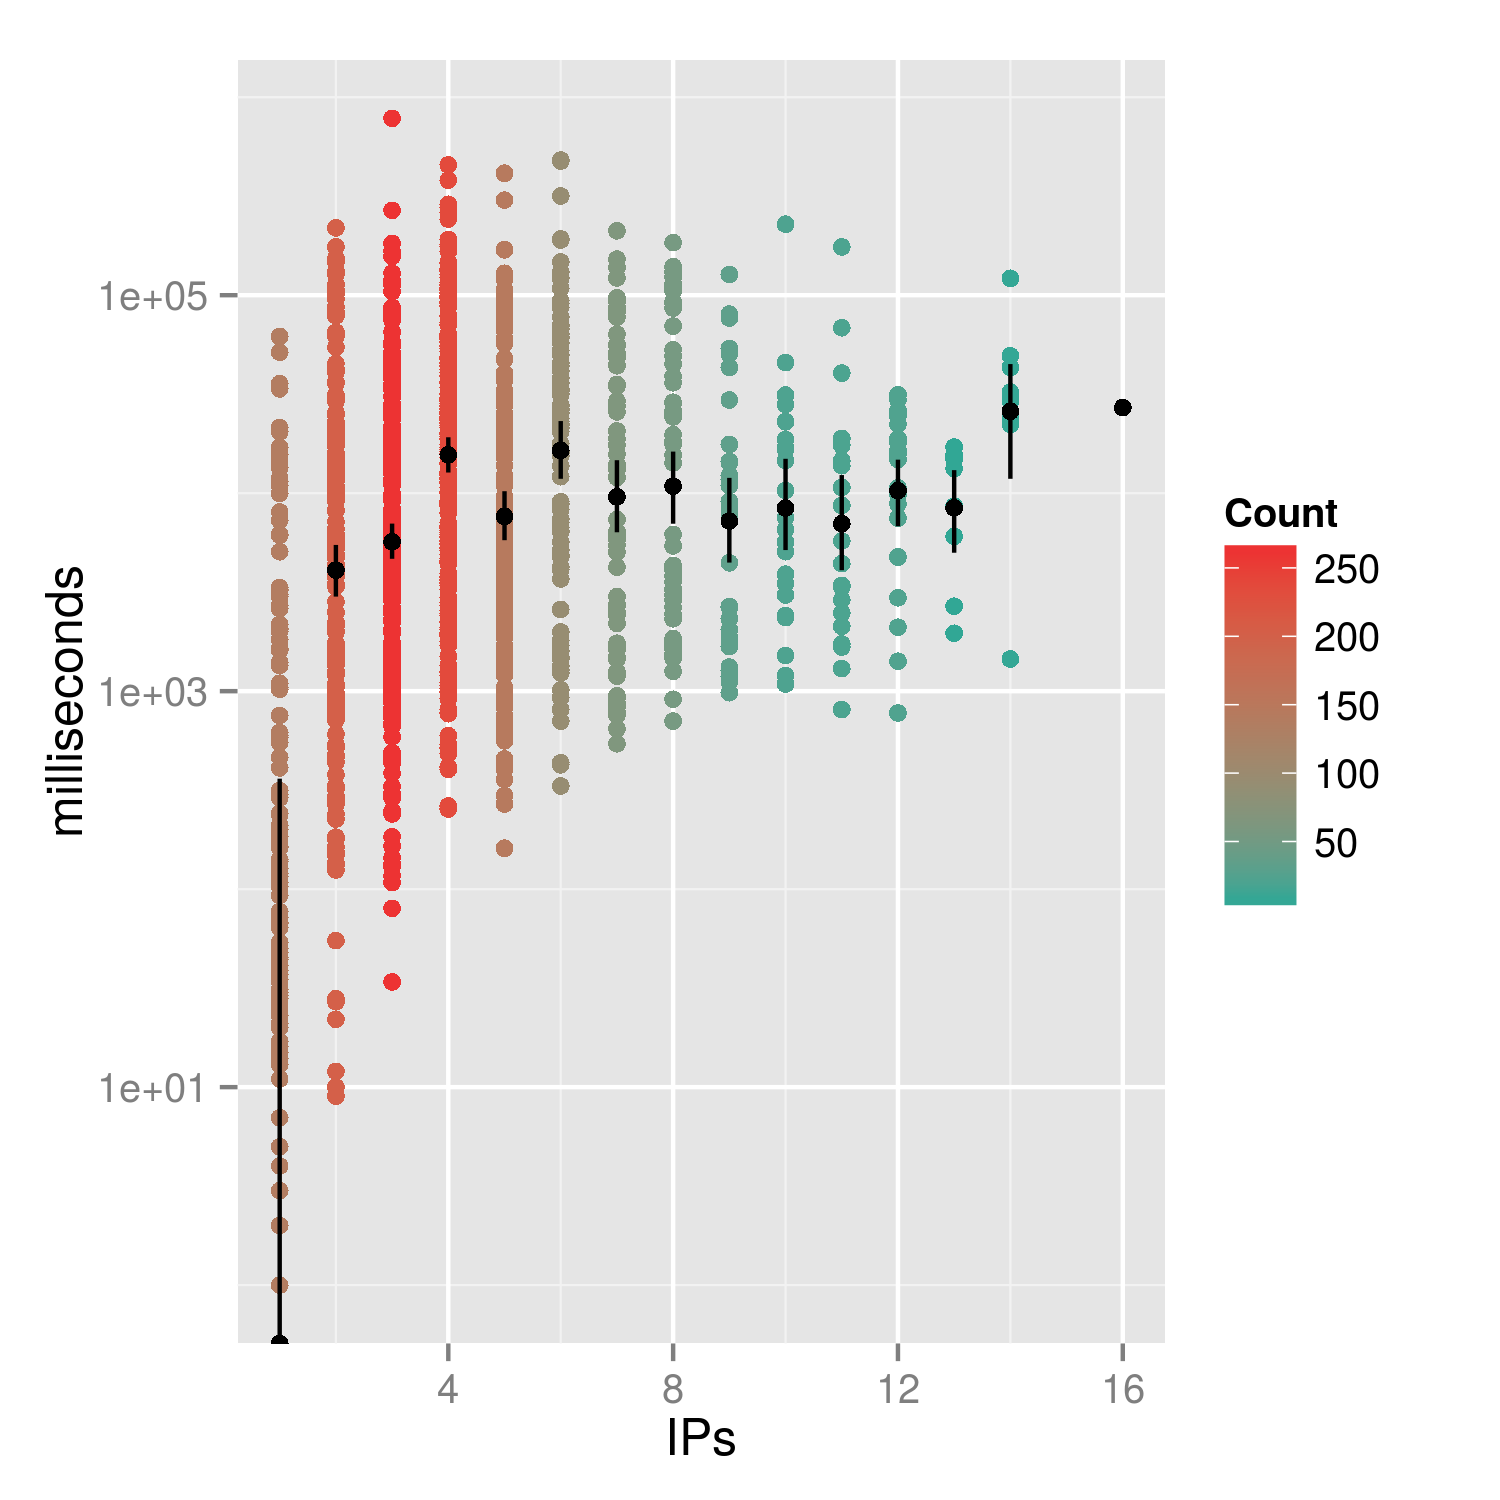
\includegraphics[width=0.9\linewidth]{ips-time-ww.png}
\caption{Time employed in every experiment vs. number of IPs (in
  abscissas). The black dot and line show the average and standard
  deviation, the blue to red shades the number of experiments with the same
  number of IPs. } 
\label{fig:ipstime:w2}
% ../data/time-vs-IPs.R 
\end{figure}

\subsection{Experiments using web workers}
\label{sec:w2}

The results reported above indicated that we should look for a way of
increasing the time users spend on the page. This led us to create an
architecture that uses web workers, which is described in
\cite{2016arXiv160101607Manom} and we abbreviate to {\sf
  NodIO-W$^2$}; web workers work in the background even if
the web page is not in focus. A few improvements were also tested,
basically using a random population and restarting the web worker when
the solution was found.

The experiments were run in the same way as before, using several
 announcements in Twitter throughout several days by the end of July
2015. Eventually, more than one thousand experiments were completed in
a matter of days. A summary of results is shown in Table
\ref{tab:summary:ww}, comparing it with the aggregate of the results
obtained with the initial version of {\sf NodIO}. These results are
remarkably different, being similar only in the median and maximum
number of IPs, although in this case it would be combination
IP-worker, as we considered every worker as a unique IP. The median
number of seconds is almost 80\% better than the previous version, and
the median number of PUTs is three times better; this causes that most
of experiments take less time than one of the baselines, and one third
less than the second baseline. Thus, the conclusion in this case is
that we can obtain, through volunteer computation, a result that most 
of the times is better than we would by using a similar, non-parallel,
desktop setup, which makes this system suitable for massively
distributed evolutionary algorithms.
%
\begin{table}
\caption{Summary of fit to GEV and Weibull distribution of
  the number of PUTs per worker. \label{tab:puts:ww}}
\begin{center}
\begin{tabular}{cccc}
\hline
Distribution & Location $\mu$ & Scale $\sigma$ & Shape $\xi$ \\
\hline
GEV & 18.275 $\pm$ 0.837  &  25.96  $\pm$ 1.22 & 1.242   $\pm$ 0.047 \\
Weibull & ND & 75.11 $\pm$ 2.97  & 0.697 $\pm$ 0.014 \\
\hline
\end{tabular}
\end{center}
\end{table}
%

However, it is interesting to note why this is so, and the first hint
is the inter-experiment correlation between the number of IPs in
successive experiments. While before it was an unremarkable 10\%, it is
now more than 43\%, making the number of IPs in contiguous experiments
highly correlated. The main reason for this is the setup in the
version using web workers, which restarts an island after a solution has been
found and also that it keeps running even if the tab is not on the
foreground. This means that volunteers can leave the experiment
running for as long as they want and they will be contributing 
experiment after experiment, unlike the previous version, where they
stopped contributing after one solution was found. This is also
reflected in the number of PUTs, more than 50\% of the volunteers run the experiment for more than
4000 generations. All things considered, this means than there are
%Mario: many more more threads {\em simultaneously} running?
more threads and many more computers {\em simultaneously} running,
leading to this almost 5-fold increase in running time.


We are also interested in measuring the scaling properties of this
model, that is, the relationship between the number of IPs
participating in an experiment and the time it takes to complete
it. This is shown in Figure \ref{fig:ipstime:w2}, which displays every
experiment in terms of time (in milliseconds) vs. % (Paloma) Isn't "vs." informal?
the number of workers participating
in it. Although there is not a clear trend, the graph seems to say
that the time needed for finding the solution in this evolutionary
algorithm does not depend on the number of workers participating in
it. This does not mean that it is independent on the number of {\em
  simultaneous} users, which is probably the case although it is more
difficult to measure. There seems to be a trend towards a decreasing
standard deviation in the time, with more volunteers adding both {\em
  robustness} to an experiment, and certainty in the time it is taking. % (Paloma) Should "certainty" go in italics? Otherwise it's confusing. 
 However, more experiments would be needed to check this hypothesis.

\begin{figure}[!htb]
\centering
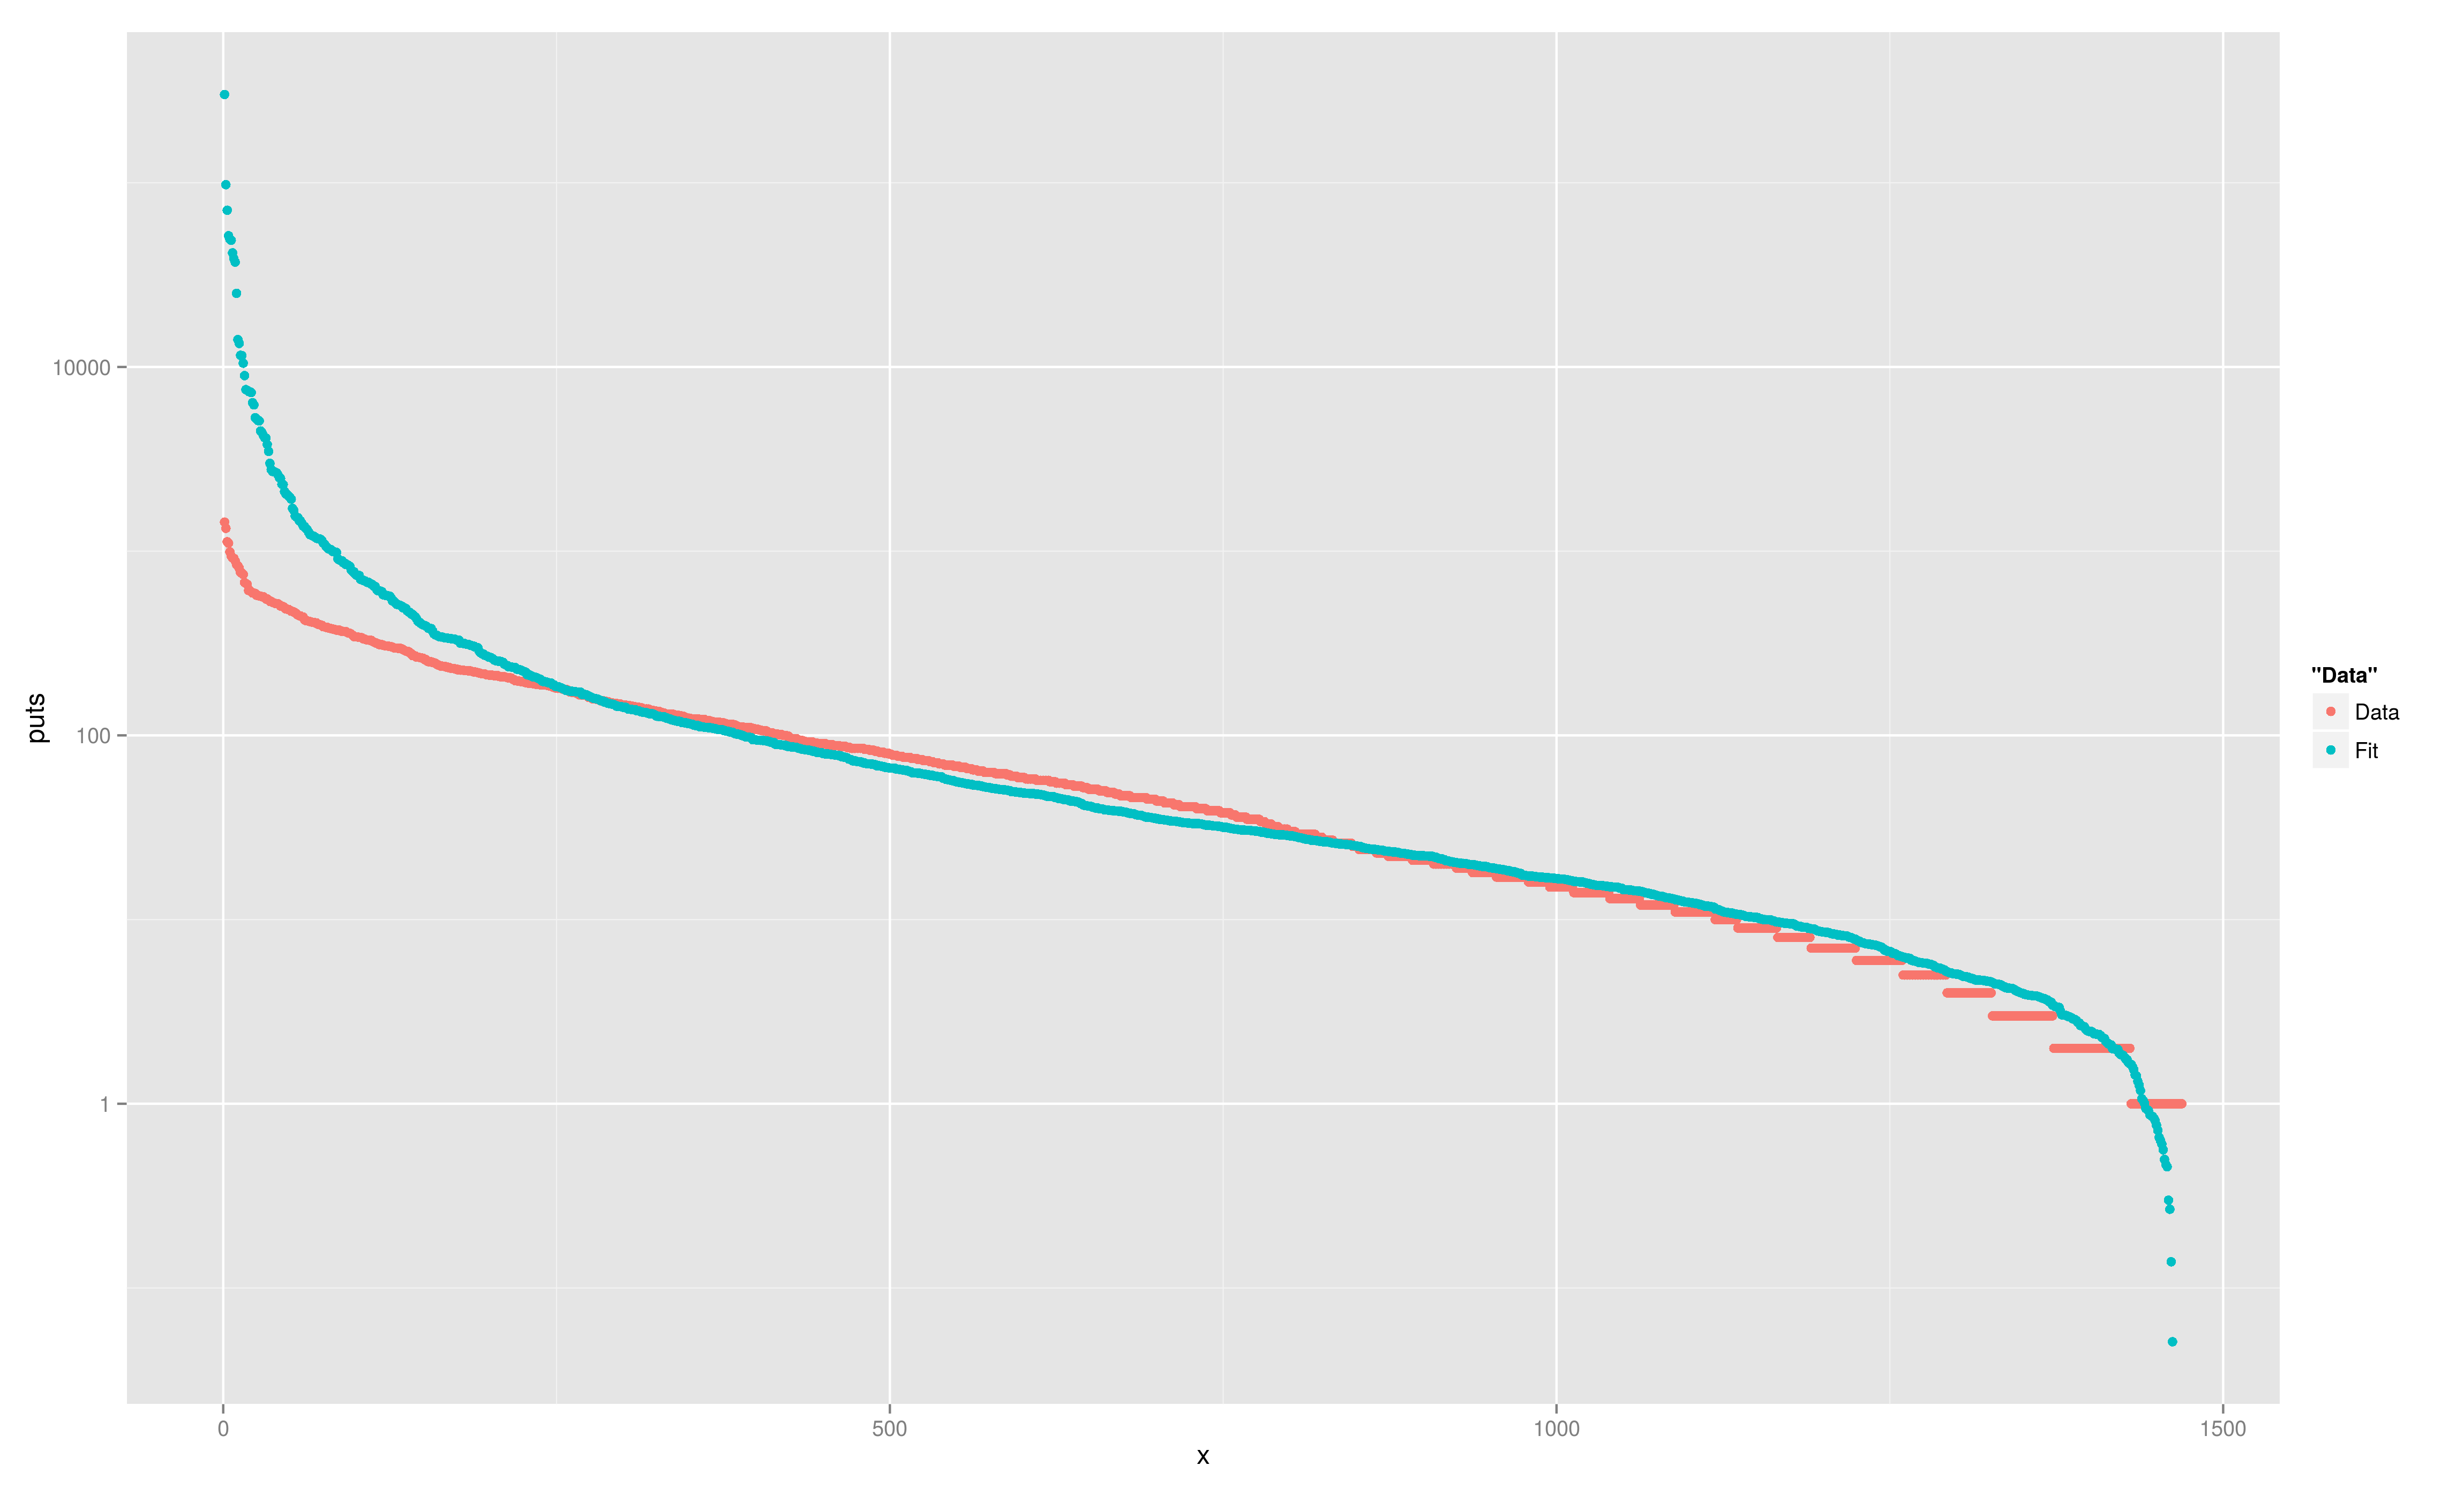
\includegraphics[width=0.49\linewidth]{gev-fit-ww.png}
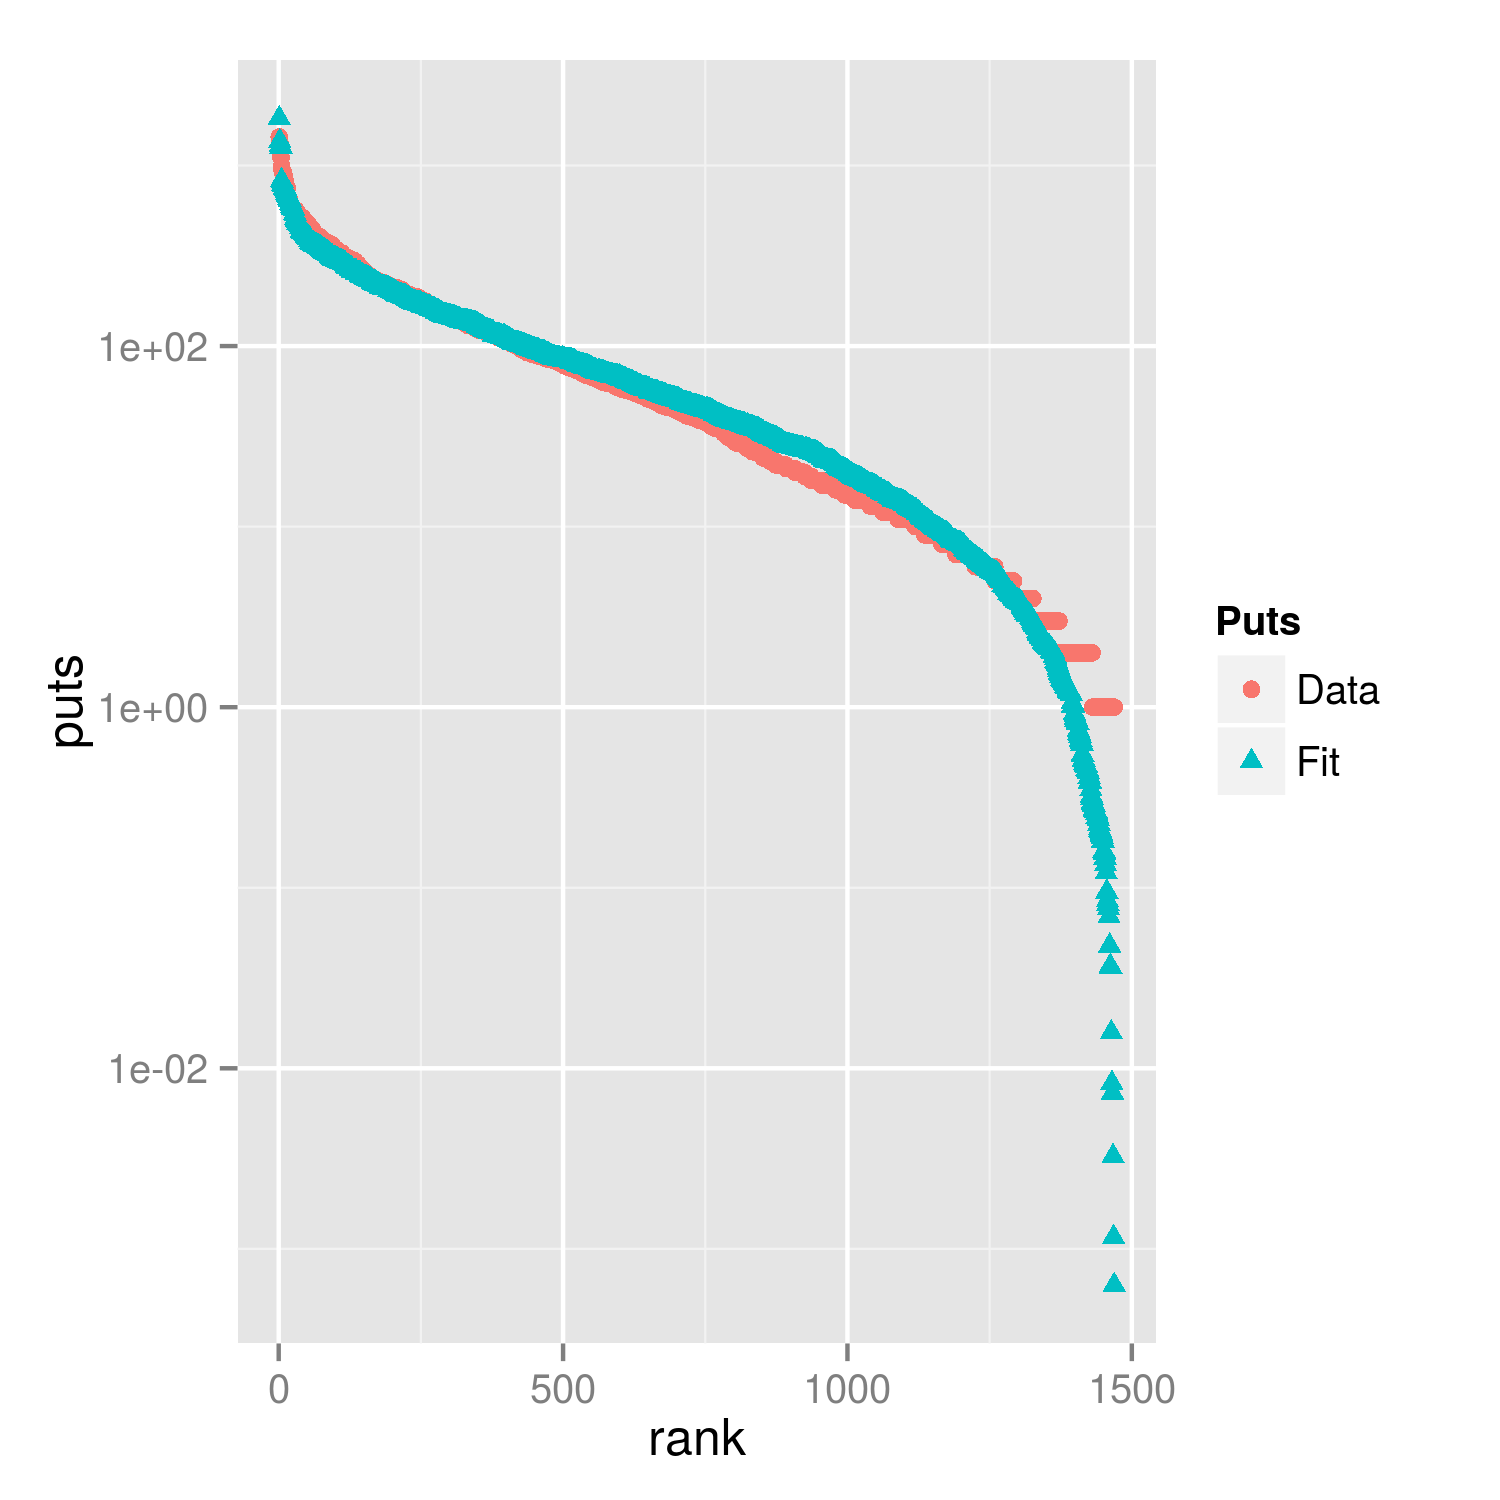
\includegraphics[width=0.49\linewidth]{weibull-fit-ww.png}
\caption{Ranked number of PUTs per worker and GEV fit (in light
  or blue color, left) 
and Weibull (in lighter or blue shade, right) for the {\sf NodIO-W$^2$} model.}  
\label{fig:gev:w2}
% File ../data/ips-puts.R
\end{figure}
%
As we did in the previous subsection, we have also fitted the number
of HTTP PUTs per worker to a  Generalized Extreme Value (GEV) function, with the result shown
in Table \ref{tab:puts:ww}. Comparing this table with what we obtained
in the previous experiment, Table \ref{tab:puts:os}, we find higher values
for the location $\mu$ and scale $\sigma$ parameters, accounting for
the higher number of contributions per volunteer that has been
previously observed. However, the shape $\xi$ parameter is
substantially similar, with a {\em bell} shape leaning towards the
origin, indicating a pattern of a few users with many contributions
and many with few contributions. If we plot the model and the data
side by side, as shown in Figure \ref{fig:gev:w2}, we see that the fit
is not so tight as in the previous case, with the model overestimating
the number of individuals with a high number contributions. This is
probably due to the fact that in the previous case the user needed to
voluntarily reload the page to contribute the most generations, with a
{\em phase change} between the people that did so and the people that
just ran the experiment once until completion. In this case, however, the
user just needs to let it run, without that phase change and thus we obtain a
more {\em egalitarian} distribution of contributions, which rather
corresponds to a Weibull function, as shown in Figure
\ref{fig:ipstime:w2} (right hand side). The fitted parameters for this
distribution, shown in Table \ref{tab:puts:ww}, show a shape parameter
equal to 0.69, a value that is remarkably similar to the 0.5 value
found for time devoted to games in Chambers et
al. \cite{chambers2005measurement}. It is important to note that, in
this case, the number of PUTs made per client does not correspond to a
uniform amount of computation, since 100 generations with a random
population belong, in each case, to different number of
operations. In other words, the same number of PUTs will correspond to
different number of operations in each case. However, since clients
are also different and take a different time in each case, it is
difficult to ascertain how this might have an influence on the
statistical distribution.

In general, this second version of the {\sf NodIO} framework and the
single experiment performed prove that it can be the foundation for a distributed
high-server-performance evolutionary computation platform,
providing reasonable algorithmic performance and being, in general,
easy to use with a straightforward modification of the fitness
function. 

\subsection{A hard optimization problem: A Shifted Rotated Rastrigin's function}
\label{sec:rastrigin}

% (Paloma) I would propose as section title "A hard optimization problem: The Shifted Rotated Rastrigin's function"

The fact that the solution of this particular problem was found in a
few seconds and restarts were necessary yielded interesting results, % (Paloma) Where?
but we needed to work on a harder problem, that is why created a new
client version that optimized a harder variation of the Rastrigin's function, 
used as a benchmark in evolutionary
algorithms. The set up for this function, and a comparison of the
baseline speed for JavaScript in a standalone experiment and other
languages is shown in \cite{2016arXiv160101607Manom}, where the details of
the implementation have also been extensively described. 

Specifically, this experiment was deployed in a virtual private server with 512MB of memory
running Ubuntu OS version 14.04 and hosted in DigitalOcean.com. Unlike previous
experiments where the optimum was expected to be found many times, 
this problem was expected to constantly run for many days finding only
sub-optimal approximations. In order to achieve this, the only change needed 
in the framework was to limit the number of chromosomes kept in the pool. 
Previously, every PUT request which included a new chromosome increased 
the size of the pool. But in a long-running experiment this has to be avoided
in order to not exhausting the available memory. In this experiment the size
of a chromosome was 1000 double precision numbers, so that considering this
and the memory available in the server, the pool was limited 
to 10,000 chromosomes.  In order to keep this size
constant, a random chromosome was pulled out of the pool before inserting a
new one, when the pool was full. For this problem {\sf NodEO}'s {\tt chromosome-float} 
and {\tt classic-ea-float} modules were used. The parameters for the EA 
were tournament size = 3 and  population size = 500, returning exchanging a
chromosome with the server every 100 generations. Again, there were two workers in each window.
As in previous experiments, a few calls to participation were published on social networks.


%
% \begin{figure}[!htb]
% \centering
% 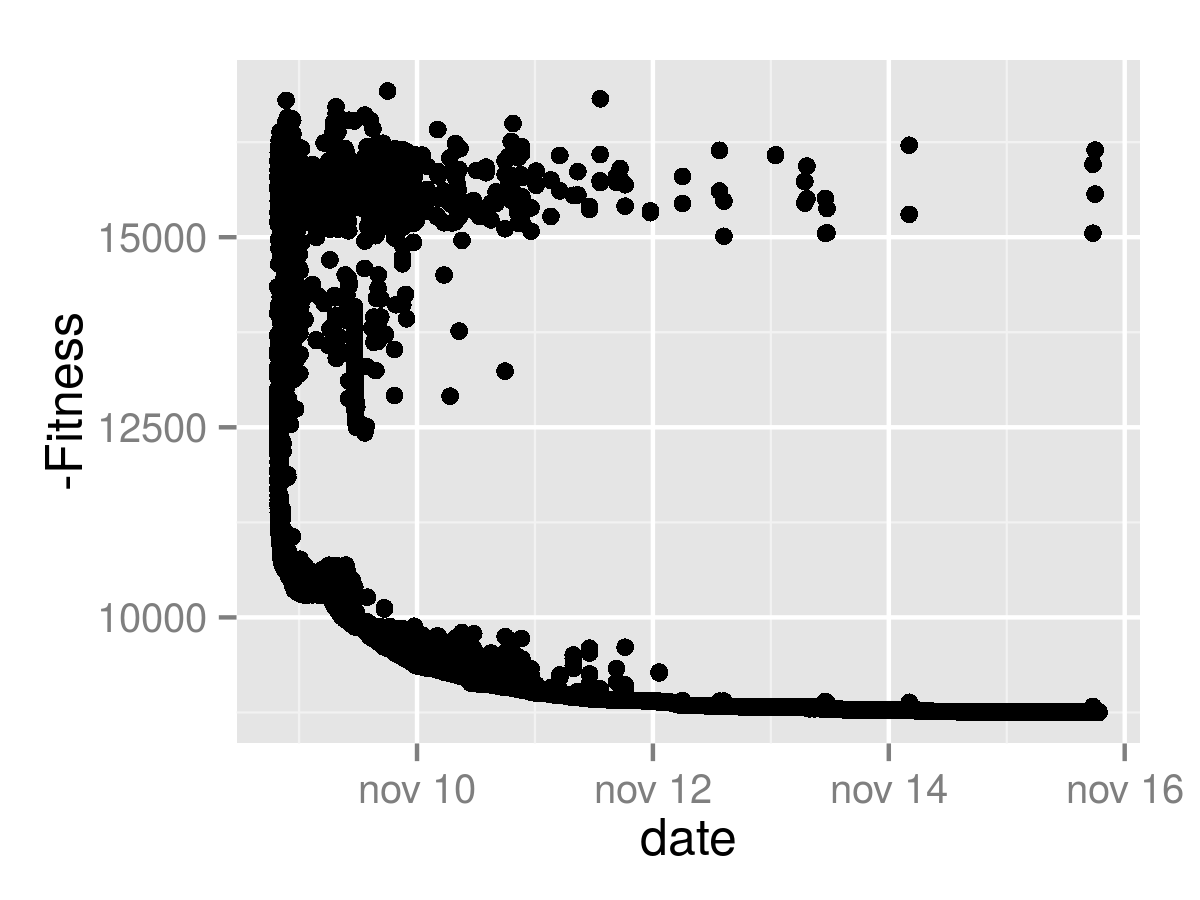
\includegraphics{rastrigin-fitness.png}
% \caption{Fitness of chromosomes sent to the server pool along time in
%   the $x$ axis.} 
% % Plotted with ../data/plot-rastrigin-fitness.R
% \label{fig:puts:rastrigin}
% \end{figure}
%
\begin{figure}[!htb]
\centering
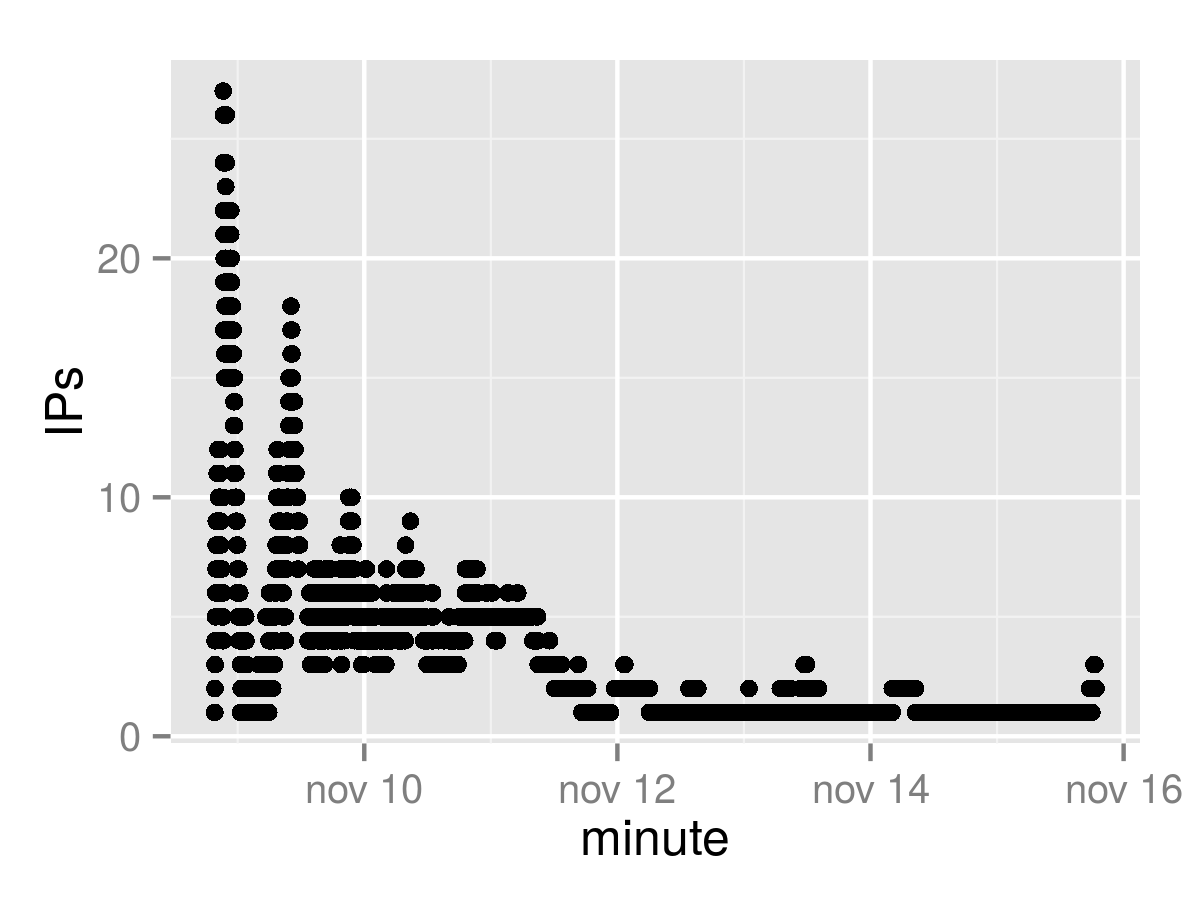
\includegraphics[width=0.49\linewidth]{rastrigin-IPs.png}
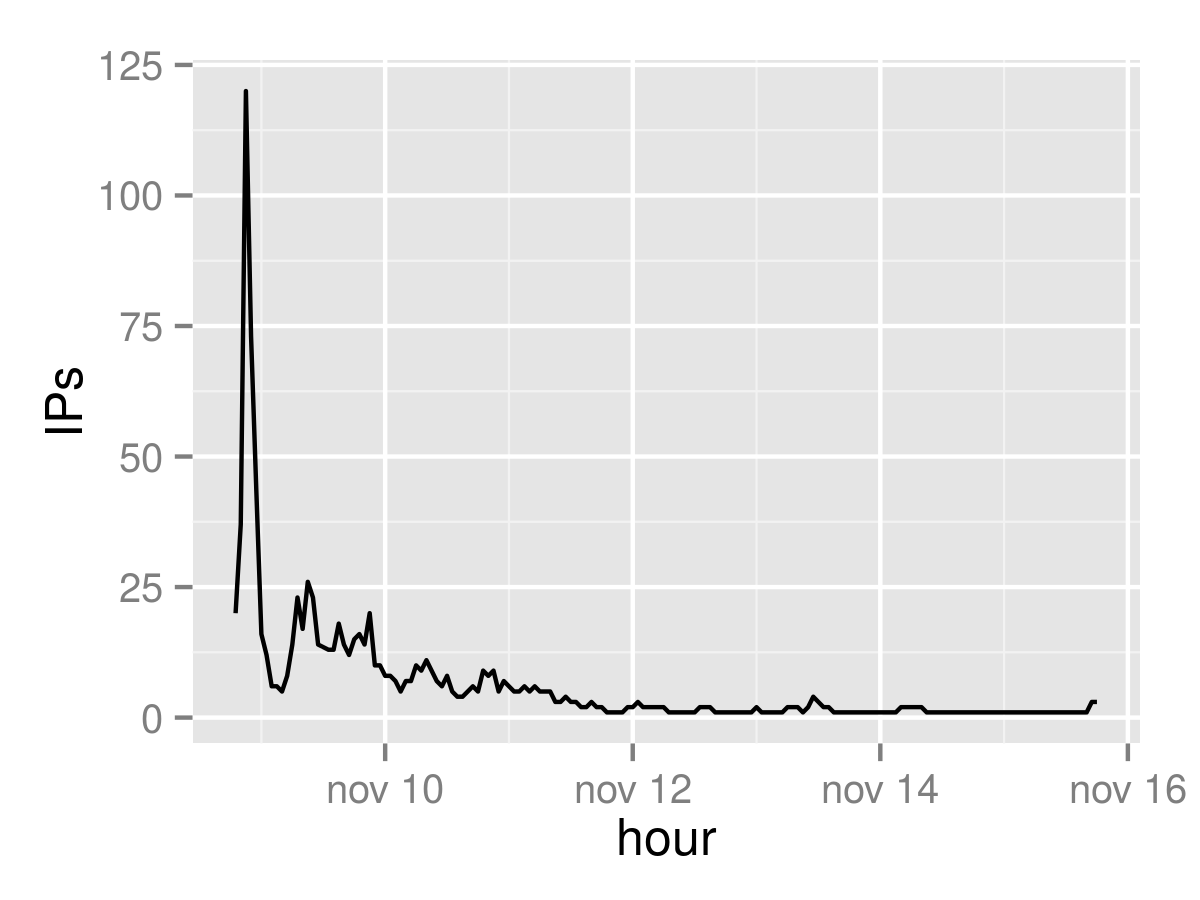
\includegraphics[width=0.49\linewidth]{rastrigin-IPs-hour.png}
\caption{Number of unique IPs participating in the Rastrigin
  experiment per minute (left) and per hour (right)} 
% Plotted with ../data/plot-rastrigin-IPs.R
\label{fig:ips:rastrigin}
\end{figure}
%
\begin{table}
\caption{Summary of fit to GEV and Weibull distribution of
  the number of PUTs per worker for the F15 (Rastrigin) function. \label{tab:puts:ww:f15}}
\begin{center}
\begin{tabular}{cccc}
\hline
Distribution & Location $\mu$ & Scale $\sigma$ & Shape $\xi$ \\
\hline
GEV & 35.759  &  343.336   & 9.877 \\
Weibull & ND & 29.00 $\pm$ 2.15  & 0.40 $\pm$ 0.01 \\
\hline
\end{tabular}
\end{center}
\end{table}
%
\begin{figure}[!htb]
\centering
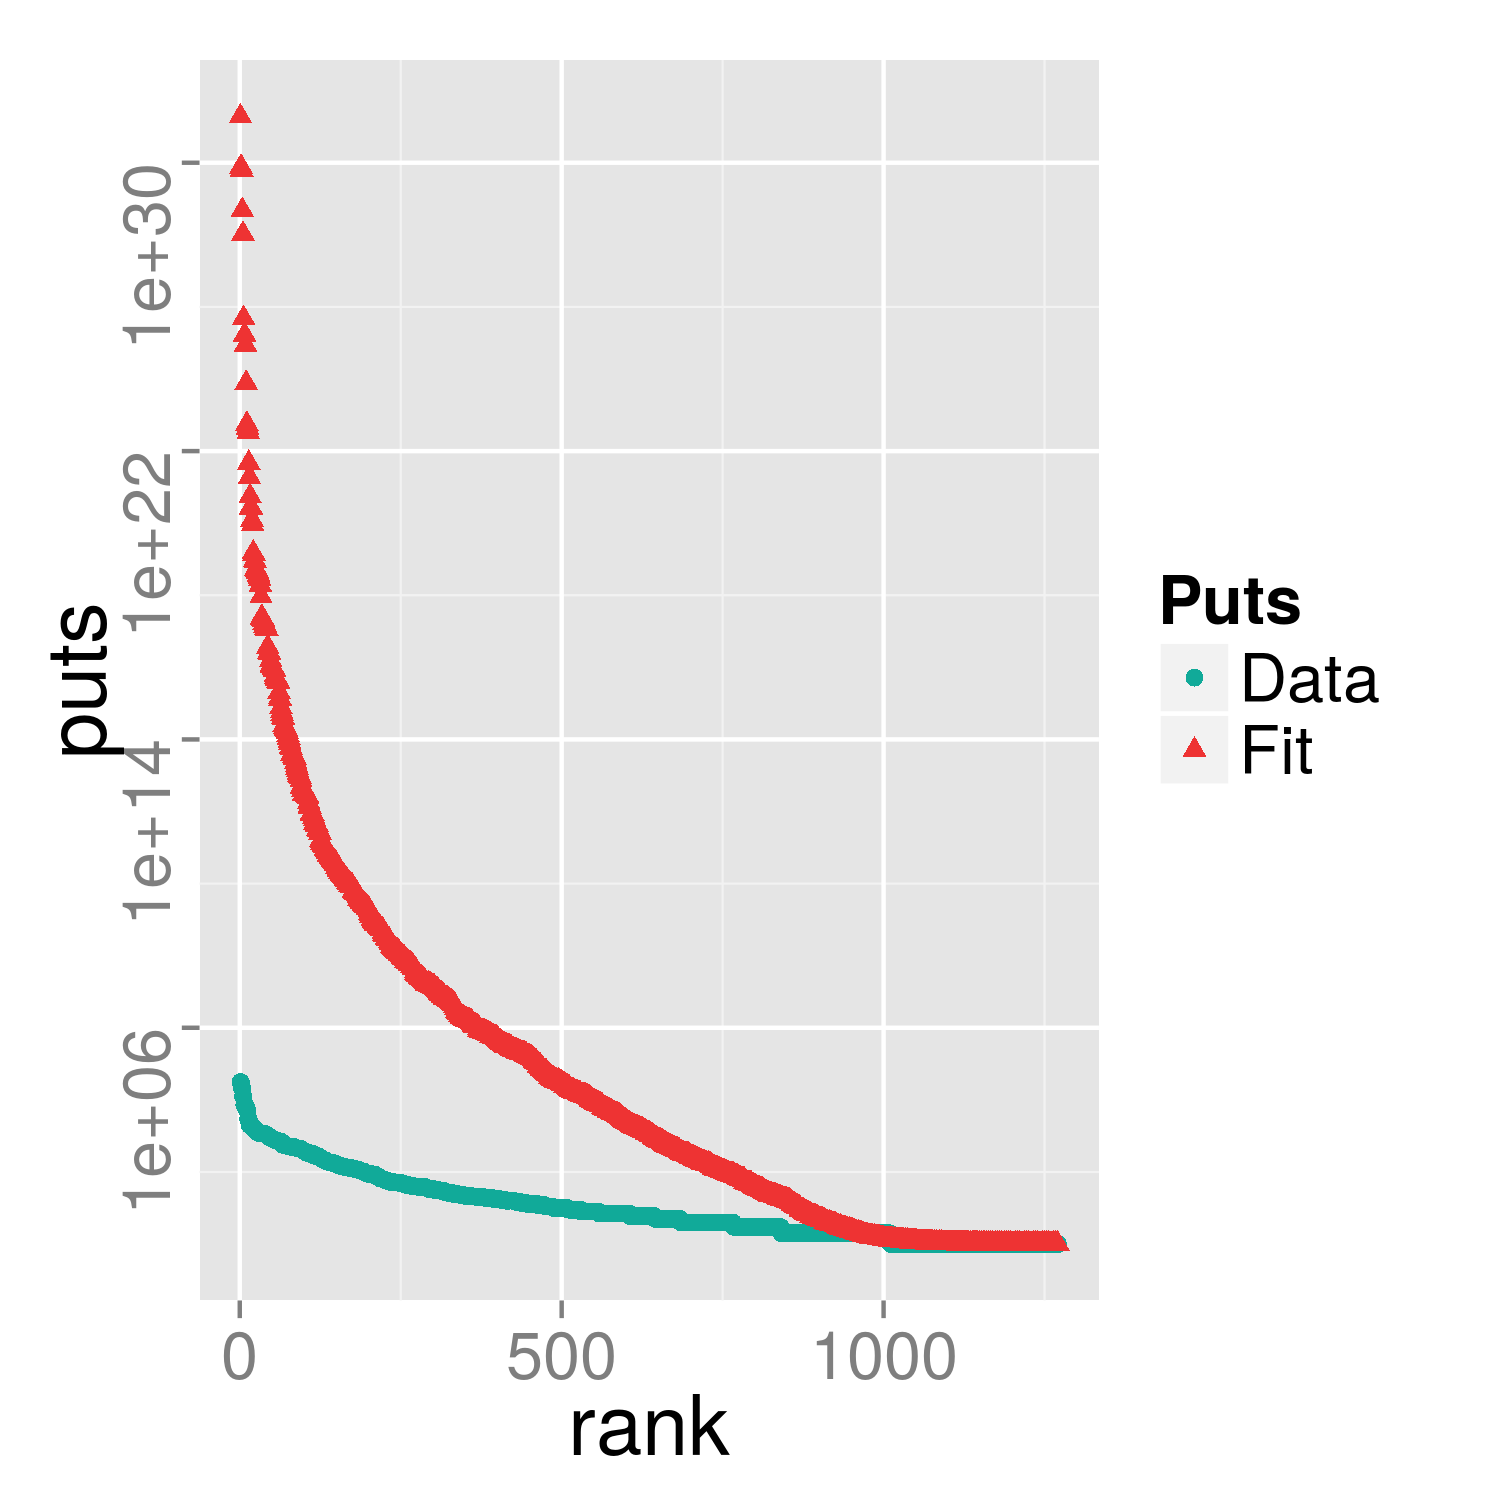
\includegraphics[width=0.49\linewidth]{gev-fit-ww-rastrigin-workers.png}
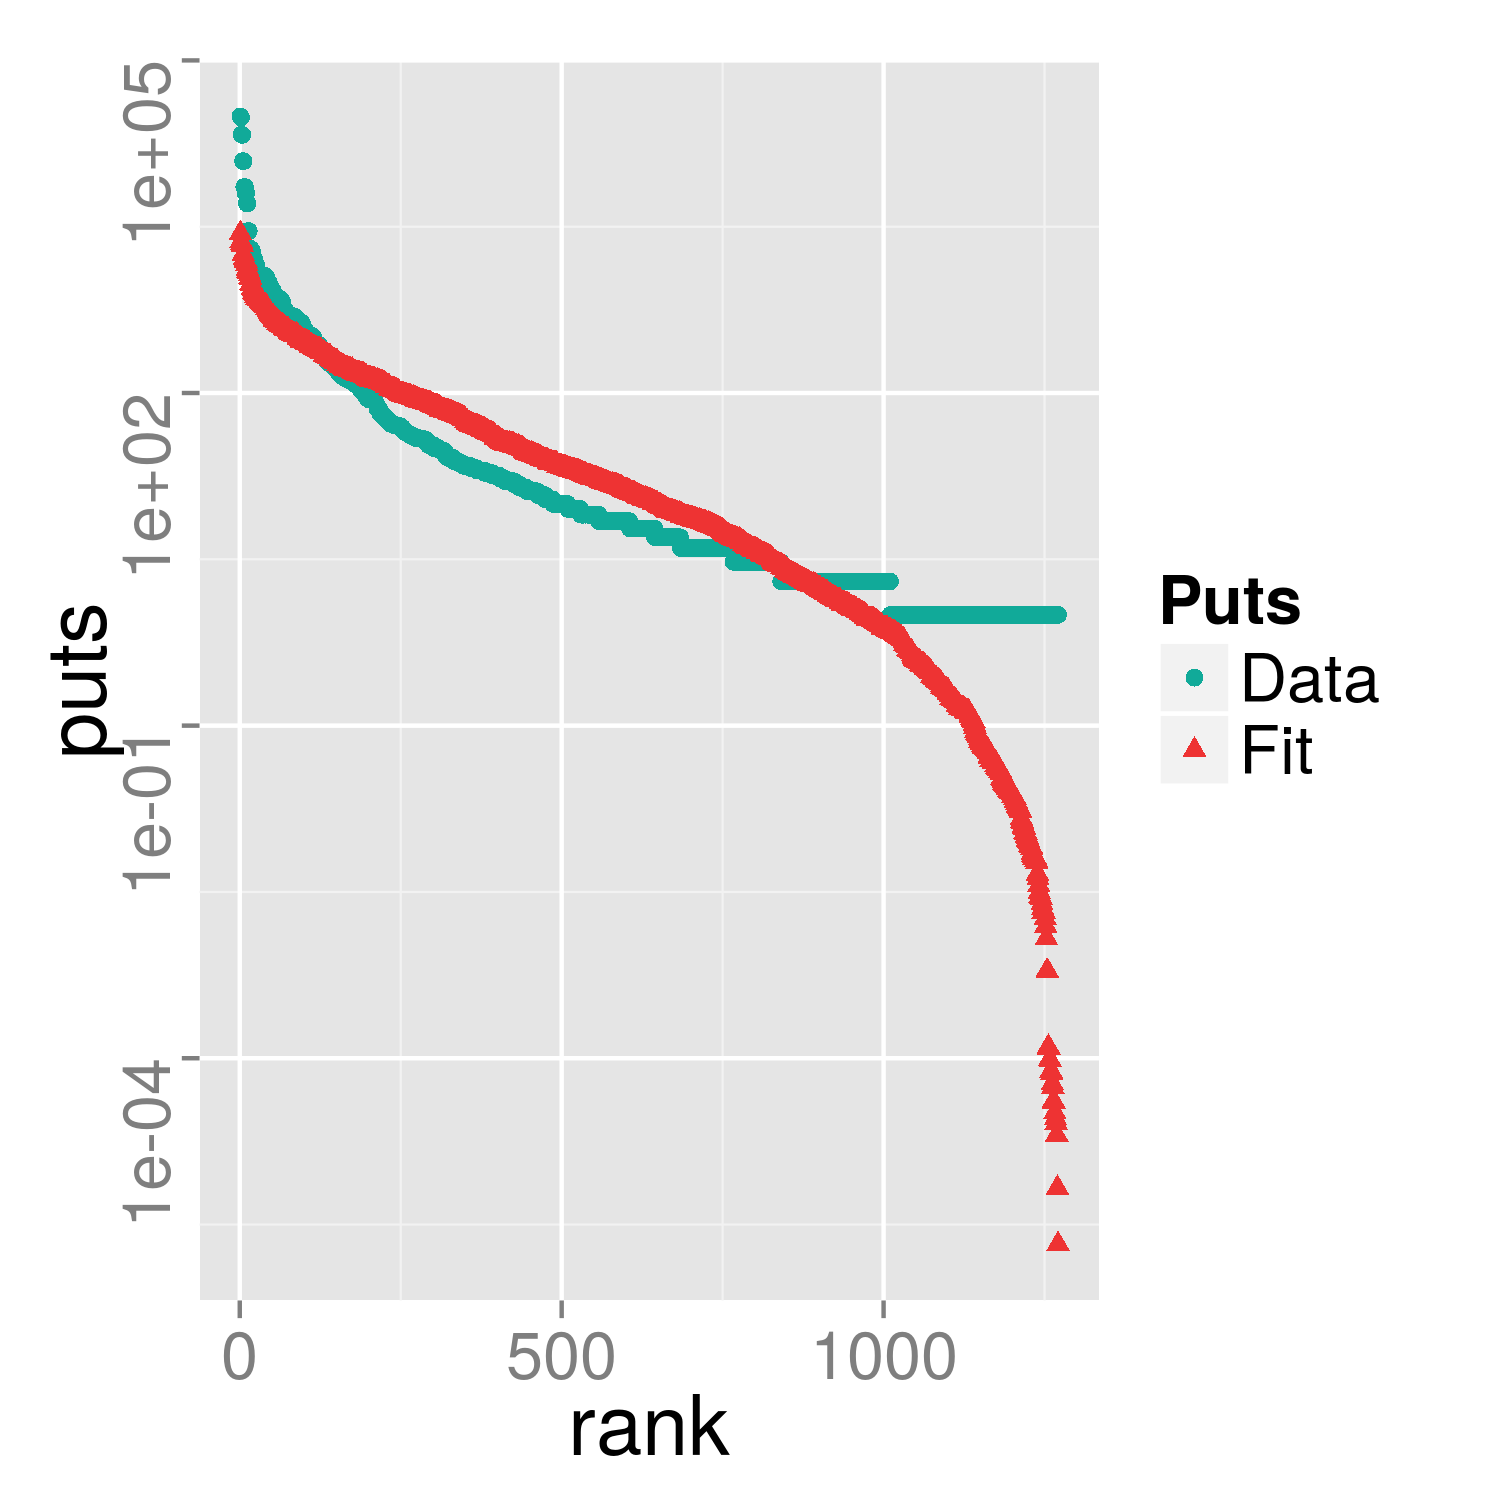
\includegraphics[width=0.49\linewidth]{weibull-fit-ww-rastrigin-workers.png}
\caption{Data and fit to GEV (left) and Weibull (right) of the number
  of PUTs per worker for the F15 (Rastrigin) function.}  
% Plotted with ../data/ips-puts-rastrigin.R
\label{fig:fit:rastrigin}
\end{figure}
%

The results for this new experiment have been extremely interesting
and quite different from the others. The most important
characteristic that sets this experiment apart is
the fact that it did not find the solution for the time it was
running, instead lowering, little by little, the fitness until it was
disconnected. The fitness of chromosomes sent by clients managed to
surpass the 9000 value by the end of the execution; and although initially there
was a high number of new nodes, this number decreased with time.

This is in part due to the fact that the presence of nodes is not
constant, as shown in Figure \ref{fig:ips:rastrigin}, which plots the
number of unique IPs participating in the experiment per minute (left)
and hour (right). The two graphs have the same shape: At the beginning there are very few or only
one, but later one there are peaks of almost 30 unique machines a
minute; these peaks appear again when new announcements are made in
Twitter or any other social networks, to go down to a few remaining
nodes later on. It is interesting to note that, at the most, more than
100 unique nodes were participating in the experiment during one hour;
also that there are sustained peaks during a day of 6-7 computers
every minute. This is due to the fact that the computation is
asynchronous, but also to the fact that different computers stay in
the simulation for a different period of time. This period has been
plotted in Figure \ref{fig:fit:rastrigin}, that plots the number of
PUTs per node, ranked by number, along with a fit to the two
distributions we have used before, GEV and Weibull; the parameters of
this fit are shown in Table \ref{tab:puts:ww:f15}. Unlike the previous
experiments, in which GEV fit was relatively good, in this case it is
quite obviously not. However, the fit to the Weibull distribution,
shown at the left of the image, is relatively good. As should be
expected, the shape and scale are different to the one in the previous
experiments with the Trap function, however, the shape is quite
similar (0.40 vs 0.69), being in both cases less than one, which
indicates a decreasing distribution of the same kind. In fact, the
difference in the scale parameter indicates that the difference
between the time devoted by a volunteer and the next is bigger in this
case. This is probably due to the fact that the duration of the
experiment is bigger, allowing for bigger differences in
behavior. While the first in the Trap function might have devoted a
few minutes and the second a few seconds less, the difference between
the first and second in this experiment might be in the scale of
hours. 


In general, this experiment confirms what was found in the others in
several aspects: first, there is a regularity in the distribution of the
time assigned by volunteers to it, second, there is a good and certain
amount of volunteers that will become part of the distributed
computer, in some cases up to one hundred; also, in some cases there
will be users that will spend several hours, two orders of magnitude
more generations in this case than in the previous one.
%Mario: than in the previous one. Are we refereing to the Wˆ2 version?
There is a clear influence of the time to solution: a short time means that every
experiment will only gather a few volunteers, but also that they will
stay only for a short time. A long time will make users stay for
longer, but if it takes too long, they will eventually lose interest. 

We will discuss this and the rest of the findings of the paper in the
conclusions. 

%---------------------------------------------------------------
\section{Conclusions and future work}
\label{sec:conclusion}

In this paper several experiments with a client-server architecture for volunteer and distributed
evolutionary algorithms have been performed. The architecture uses the
browser and has been generated using the {\sf
  NodIO} framework, which includes  {\sf NodEO} as an evolutionary
algorithm library. Volunteers are {\em in the cloud}, as stated in the
title, 
since they are a {\em CPU as a service} for the persons running the
experiment. In fact, in this paper we have tried to put some figures
on the real size of that {\em cloud} in case it is used by itself or
in conjunction with other local or 
cloud-based methods to add computing power in a seamless way through
the pool that {\sf NodIO} creates. 

In order to establish a baseline performance, which was published in
\cite{2016arXiv160101607Manom}, the evolutionary algorithm was run in a desktop client application written in JavaScript
using NodEO to solve the 40-trap function. The first experiments in a
volunteer computing scenario proved that, although obtaining better performance than the
baseline  was possible, it did not happen, mainly because of the
difficulty in carrying over other experiments to volunteers when the
experiment they were participating on was finished. This has been shown in the low
correlation between the number of IPs in successive experiments, and
also resulted in a low number of generations allotted by users.  

In the second implementation, Web Workers
were used so that several clients per browser page could be executed and
run in the background; our intention was to increase the time spent by
the users and, in fact, the number of generations per
user increased to the point that we obtained a performance better than
baseline in most cases. The architectural changes led to a high correlation
between successive experiments, so that, even as the median number of
volunteers per experiment decreased, they were probably contributing
to the experiment simultaneously, so that our objective was
achieved. In general, one of the first conclusions of this paper is
that the browser technologies should be used to its full extent, so
that the user time is leveraged to its full potential, and this was
achieved using web workers. 

The second objective of this paper was to model the user behavior in a
first attempt to try and predict performance. As should be expected,
the model and its parameters depend on the implementation, with contributions following
a GEV distribution with single-thread and a
Weibull distribution when web workers are used. These distributions are
close enough to each other and, in the second case, reflect the fact
that most time spent in the page is actually devoted to computing, as
opposed to presenting the chart or not doing anything,
which is why the time spent (represented by the number of
contributions to the pool) follows a model quite similar to that found
for games or other online activities. The reverse implication, from
games to volunteer computing,  might also be true: if we
want to have returning users for the experiments, it is probable that
we should {\em gamify} the experience so that once they have participated
once, they would be encouraged to do for a longer time or to share
it. In the spirit of Open Science, this 
gamification might involve computing in real-time data such as the one
presented in this paper, while showing it in the same page. 

In general, linking and finding correlations between user choices and
performance is an interesting avenue to explore in the future. % (Paloma) Mario, isn't this the future work? Should it be in conclusions? If not, just ignore this comment.
% Moved to conclusions. 
There are several validity threats to the design of this study.
Participants of the experiments were mainly members of our 
own social networks, personal colleagues, friends 
and acquaintances, therefore, to extend this work other options 
should be considered in order to include 
a wider audience with different motives for participation.
Another threat is that participants were anonymous, so the amount of repeated 
participations and the effects this might have had in the outcome is not
known. Another issue is that the scalability of the system was not thoroughly tested
but for the amount of participants the basic configuration 
was more than adequate, then again more experiments are needed in order
to assess the capability both with more clients and other server
configurations. Although care was taken to include representative benchmarks
of real world problems, more experiments with a broader coverage 
should allow a better understanding of the practical limitations of
the architecture and the tools chosen.
%  Even if
% the three previous experiments were published in a similar way, one
% obtained up to 5 times more total cycles  than the one with the least
% number of cycles. 
It is also essential to obtain volunteers as
simultaneously as possible, so it is possible that the features of the
social network in terms of real-time use will also play a big
role. Even as it is difficult to create controlled experiments in this
area, it is an interesting challenge to face in the future. % (Paloma) Wrong collocation

This paper also shows that the time needed to find a solution or if it
is eventually found have an influence on the time people devote to
it. It would be so interesting to check the performance for other computationally demanding
tasks, especially ones that cover the middle ground between a problem
finishing in seconds or minutes (Trap) and weeks (Rastrigin F15). 
Besides, the two versions of the framework include as an
algorithmic variant using random population size. We do not think this
has had a big influence on the results and in fact this is not noticed
for F15, which is the last version tested, but it would be interesting to
measure exactly what this influence has been. 
% In general there are
% many issues with the evolutionary algorithm implementation itself,
% including using different, or adaptive, policies for inserting and
% sending individuals to the pool as was done in \cite{araujo2008mam},
% using different policies for population initialization, and also the
% incorporation of high-speed local resources to the pool to check what
% would be the real influence of the volunteer pool to the final
% performance. 

Other improvements could include adding a bit of more
control to the user might contribute also to gamification. Right now
the user has only two Web Workers. It is a matter of a single click to
open more tabs in the browser, giving more Web Workers, but it would be
interesting to put everything in a single page and under our control,
to check how often this happens and under which conditions. 

% Finally, the implementation needs some refinement in terms of
% programming and also ease of use. Tools such as Yeoman might be used % ¿añadir una cita o la URL http://yeoman.io/ a pie de página ?
% to create a generator in which the user just has to create a fitness
% function, with the rest of the framework wrapped around
% automatically.
%  All this, as well as the data used for this paper and the paper
% itself, has been published with a free license in GitHub at
% \url{https://github.com/JJ/modeling-volunteer-computing}.  
% Pablo: I should uncomment this last paragraph, but using the url: https://github.com/ANONYMOUS

%---------------------------------------------------------------
\section*{Acknowledgments}
 
This work has been supported in part by
TIN2014-56494-C4-3-P (Spanish Ministry of Economy and Competitivity), PROY-PP2015-06 (Plan Propio 2015 UGR), 
SPIP2014-01437 (Direcci{\'o}n General de Tr{\'a}fico) and PYR-2014-17
GENIL project (CEI-BIOTIC Granada). Additional support was recieved by
Projects 5622.15-P (ITM) and  PROINNOVA 2015: 220590 (CONACYT).

\bibliographystyle{abbrv}
\bibliography{geneura,volunteer,javascript,ror-js,GA-general}

\end{document}
%%% Local Variables:
%%% ispell-local-dictionary: "english"
%%% End:
